% \part{Temes avançats}
% \label{part:avançats}

\chapter{Gestió d'excepcions}
\label{ch:exceptions}
Sovint treballant amb sistemes encastats ens trobem amb errors d'origen desconegut que es poden provocar per múltiples causes. Així, per exemple, una divisió per zero, un accés incorrecte a una zona de memòria o un accés a una posició de memòria fora de rang faran que el processador es reiniciï \cite[102]{DesignersGuide}\cite[318]{ARMsdg}\cite{KielHardFault}.

Aquests casos poden ser molt difícils de trobar si són casos esporàdics, però l'arquitectura ARM té unes característiques que ajuden a detectar-los i trobar-los. En síntesi, el cortex-M llença una interrupció molt prioritària anomenada {\bf HardFault\_Handler()}\index{HardFault\_Handler()} quan succeeix un problema greu del que el processador no pot recupera-se, com una divisió per zero, un accés il·legal a memòria, etc. Abans de cridar a l'excepció, la CPU guarda tot de valors claus a diferents registres, i així per exemple en el registre {\bf PC} s'hi emmagatzema l'adreça de la instrucció executada, així que, en principi, només cal anar a aquella posició de memòria per veure quin ha estat el codi que ha causat el problema. També s'emmagatzema el valor de retorn (la  instrucció següent a l'executada que ha causat l'error) al registre {\bf LR} \cite{BlogHardFalut}.

Així doncs, es pot reescriure la ISR per obtenir les dades que ens informi sobre què ha passat per ajudar-nos a obtenir pistes de quin codi està fallant.\cite{ARMHandler}.

\section{Exemple detectant errors greus}
A l'\href{https://github.com/mariusmm/cursembedded/tree/master/Simplicity/ErrorHandling}{exemple del repositori} hi ha un codi que genera diferents errors segons la funció que es cridi i una implementació de {\bf HardFault\_Handler()}\index{HardFault\_Handler()}. Aquesta funció està escrita en assemblador, però el que cal veure és que es crida a la funció {\bf my\_HardFault\_Handler()}\index{my\_HardFault\_Handler()} que es qui en realitat fa tota la feina i és la que cal entendre \cite{EFM32HardFault}.

\index{my\_HardFault\_Handler()}
\begin{lstlisting}[style=customc,caption=Codi HardFault\_Handler,label=HardFaultHandler_1]
void my_HardFault_Handler(uint32_t *stack) {
  printf("Error Handler\r\n");
  printf("SCB->HFSR = 0x%08lx\r\n", (uint32_t) SCB->HFSR);

  if ((SCB->HFSR & (1 << 30)) != 0) {
    printf("Forced Hard Fault\r\n");
    printf("SCB->CFSR = 0x%08lx\r\n", SCB->CFSR);

    if ((SCB->CFSR & 0x02000000) != 0) {
      printf("Divide by zero\r\n");
    }
    if ((SCB->CFSR & 0x01000000) != 0) {
      printf("Unaligned\r\n");
    }
    if ((SCB->CFSR & 0x00010000) != 0) {
      printf("Undefined\r\n");
    }
  ...
}
\end{lstlisting}

A la primera part (veure Llistat~\ref{HardFaultHandler_1}) de la \gls{ISR} es treu per la consola de debug la causa de l'excepció ({\em bus fault}, {\em memory access}, {\em divide by zero}, etc.).

Tot seguit es treu per la mateixa consola els valors dels registres que hi ha a l'\gls{stack} per tenir dades que ens permetin localitzar l'error (Llistat~\ref{HardFaultHandler_2}).

\begin{lstlisting}[style=customc,caption=Codi HardFault\_Handler,label=HardFaultHandler_2]
void my_HardFault_Handler(uint32_t *stack) {
  ...
  printf("sp = 0x%08lX\r\n",  (uint32_t) stack);
  printf("r0 = 0x%08lX\r\n",  stack[0]);
  printf("r1 = 0x%08lX\r\n",  stack[1]);
  printf("r2 = 0x%08lX\r\n",  stack[2]);
  printf("r3 = 0x%08lX\r\n",  stack[3]);
  printf("r12 = 0x%08lX\r\n", stack[4]);
  printf("lr = 0x%08lX\r\n",  stack[5]);
  printf("pc = 0x%08lX\r\n",  stack[6]);
  printf("psr = 0x%08lX\r\n"  stack[7]);
  ...
}
\end{lstlisting}


\begin{figure}
 \centering
 \fbox{\color{ocre}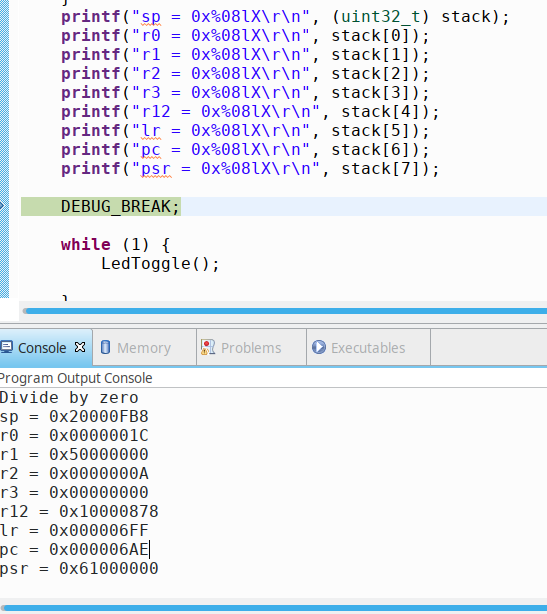
\includegraphics[width=0.65\textwidth, keepaspectratio]{imatges/HardFault_Console.png}}
 \caption{Debugger aturat a la instrucció DEBUG\_BREAK i el {\em dump} els registres}
 \label{fig:HardFaultDump}
\end{figure}


Per últim, es crida la macro {\bf DEBUG\_BREAK}\index{DEBUG\_BREAK}, que està definida com una instrucció en assemblador ({\bf BKPT \#01}) que posa el {\em core} en mode {\em Debug} i atura l'execució en aquest punt. Així, si tenim un {\em debugger} connectat, veurem com l'execució s'atura en aquest punt i torna el control a la nostra eina (veure Figura~\ref{fig:HardFaultDump}).


\begin{figure}
 \centering
 \fbox{\color{ocre}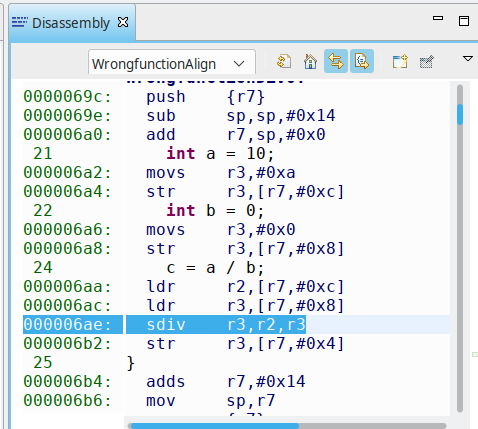
\includegraphics[width=0.65\textwidth, keepaspectratio]{imatges/HardFault_Dissassembly.png}}
 \caption{Codi assemblador a la posició de memòria indicada pel registre {\bf PC}}
 \label{fig:HardFaultDis}
\end{figure}

Si anem a la finestra {\em Disassembly} i anem a la posició de memòria que indica el registre {\bf PC} (0x6AE a l'exemple), veurem que apunta a una instrucció assemblador {\em sdiv}, que es corresponent amb una divisió. Si mirem el codi anterior, podem deduir que a la posició de memòria {\bf R7+0x8} (corresponent a la variable {\em b}) s'hi ha emmagatzemat un 0 (instruccions a 0x6A6 i 0x6A8) i aquesta variable es fa servir a la divisió com a divisor, causant l'error (veure Figura~\ref{fig:HardFaultDis}).

També cal comentar que les diferents funcions que generen errors són les següents:
\begin{itemize}
 \item {\bf WrongfunctionDiv0()}\index{WrongfunctionDiv0()} causa una divisió per zero.
 \item {\bf WrongfunctionAlign()}\index{WrongfunctionAlign()} causa un error d'accés a memòria fora d'alineament.
 \item {\bf WrongfunctionWrongMemory()}\index{WrongfunctionWrongMemory()} causa un error per accés fora dels límits de la memòria.
 \item {\bf fp()}\index{fp()} causa un intent d'executar a la posició 0x0000\_0000 de memòria.
\end{itemize}

\chapter{{\em Shadow Registers}}
En algunes arquitectures i en perifèrics d'alguns fabricants poden llegir que es fan servir {\em shadow registers}. S'anomenen així a registres que contenen una còpia d'un altre registre i que son els que es poden llegir per part d'altres dispositius o perifèrics. 

Així per exemple, trobem {\em shadow registers} a alguns processadors de manera que quan la CPU entra a una interrupció es passa a treballar amb un banc separat de registres de propòsit general. Això es fa per evitar un sobrecost a la crida de la ISR, ja que si es tenen aquests registres s'han de guardar els valors actuals de tots els registres a la pila abans de poder executar el codi de la ISR. En canvi, si es tenen aquests registres, la CPU passa a treballar amb un banc diferent (els {\em shadow registers}) durant l'execució de la ISR i no cal salvaguardar cap valor dels registres originals. Un cop se surt de la ISR la CPU torna a treballar amb el banc de registres originals. En el cas dels Cortex-M no es treballa amb aquesta mena de {\em shadow registers} i, per tant, caldrà que les ISR salvin els valors dels registres de propòsit general que sobreescriguin durant la seva execució.

Una altra lloc on ens podem trobar {\em shadow registers} és en alguns perifèrics que treballen valors grans repartits en diversos registres. Si aquests registres s'actualitzessin entremig d'una lectura per part del Firmware, aquest podria tenir una inconsistència a les dades. Per això, és habitual que un valor determinat s'emmagatzemi a {\em shadow registers} mentre els registres ``amagats'' s'actualitzen de forma normal. Aquests {\em shadow registers} seran els que el firmware pot llegir i s'actualitzaran tots de cop una vegada s'hagin llegit tots pel firmware. 

\begin{remark}
 A tots ens ha passat o tenim un company que ha perdut una tarda sencera intentant llegir uns registres d'aquesta mena sense seguir bé l'ordre i rebent valors dolents sense caure en el problema amb els {\em shadow registers}.
\end{remark}

Un exemple d'això últim succeeix amb els registres de data i temps del RTC dels microcontroladors d'ST (veure~\fullref{sub:RTC}). Aquest perifèric conté uns {\em shadow registers} on es copien cada 2 cicles els registres reals amb la data, el temps i els segons del RTC (Figura~\ref{fig:ShadowRegisters}). Quan es llegeix el registre amb el temps o amb els segons es bloqueja la còpia de tots els tres registres perquè la lectura dels demès no doni cap incoherència. Si no hi fossin, podria passar que es llegís el temps (per exemple les 23:59:59 del dia 1) i poc després al llegir la data ja hagués passat el segon i la data ja fos el dia 2, resultant en que enlloc de llegir les 23:59:59 del dia 1 s'hauria llegir les 23:59:59 del dia 2. En aquest cas sembla que és molt millor llegir la data correcte i que es tingui un error d'un segon a tenir un dia sencer d'error (!).

Per tant, en aquest perifèric, primer cal llegir el registre amb el temps o els segons i després el registre amb la data \cite[800-805]{STM32F4RM}. Així si només es vol llegir el temps del RTC perquè no interessa la data del sistema, no es poden fer lectures consecutives del temps sense llegir també, encara que no interessi, la data del RTC. La API del fabricant en aquest cas no ho gestiona, però si que ho adverteix a la seva documentació \cite[719]{STM32UM1725}.

\begin{figure}
 \centering
 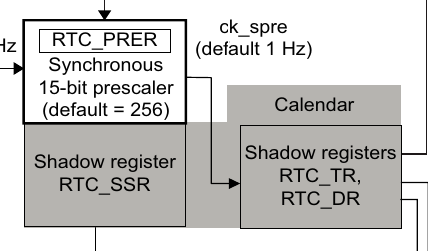
\includegraphics[width=0.65\textwidth, keepaspectratio]{imatges/ShadowRegisters.png}
 \caption{{\em Shadow registers} del perifèric RTC dels STM32 \cite[800]{STM32F4RM}}
 \label{fig:ShadowRegisters}
\end{figure}


\chapter{Baix cosum}
\label{ch:low-power}
Un dels temes més habituals de trobar-se quan es tracten temes amb microcontroladors és el del baix consum. Gràcies a la tecnologia de fabricació dels microxips i els avenços en les arquitectures dels microcontroladors, aquests han arribat a unes fites de consum molt baixes, permeten desenvolupar aplicacions on el sistema pugui anar alimentat per bateries o altres fonts d'alimentació alternatives a l'alimentació general. En aquest capítol veurem les característiques actuals dels microcontroladors en aquest aspecte, com treure tot el partit a aquestes característiques i, per últim, com adaptar els \gls{RTOS} per treballar amb baix consum.

Cal repassar uns quants conceptes sobre el consum d'energia abans d'introduir-nos de ple en el tema.

\section{Consideracions prèvies}
\label{sec:lowpowerintro}

Per la pròpia natura dels circuits digitals, aquests consumeixen sobretot quan el seu rellotge principal està actiu. Això fa que l'estratègia principal per reduir el consum d'un circuit és desactivar-li precisament el rellotge o reduir la seva freqüència, ja que el consum és proporcional a la velocitat de rellotge.
\begin{remark}
 Donat que el consum és quasi proporcional a la freqüència de rellotge, els fabricants acostumen a donar el consum per MHz (típicament $\mu$A/MHz).
\end{remark}

També cal tenir en compte que qui més consumeix en un microcontrolador és el propi {\em core} o CPU i que, per tant, serà el mòdul que caldrà tenir apagat el màxim de temps possible.

\section{Modes d'{\em sleep}}
\label{sec:sleepmodes}
Els diferents fabricants de microcontroladors basats en Cortex-M ofereixen diferents modes d'sleep, això és, diferents combinacions de perifèrics que estan actius a cada mode per tal de reduir el consum.

Així, els microcontroladors de Silicon Labs tenen 4 modes d'sleep\footnote{A més, hi ha el mode normal, on la CPU està a ple rendiment} \cite[6]{EFM32GRM}:
\begin{itemize}
 \item EM0 - {\em Energy Mode 0}: Tot el sistema està actiu incloent-hi tots els perifèrics.
 \item EM1 - {\em Energy Mode 1}: La CPU està desactiva i la resta de perifèrics estan disponibles.
 \item EM2 - {\em Energy Mode 2}: La CPU està desactivada i només els perifèrics de baix consum estan disponibles (UART, RTC, TIMER, Watchdog)
 \item EM3 - {\em Energy Mode 3}: Tot el sistema està desactivat, només es manté la RAM activada i certes interrupcions
 \item EM4 - {\em Energy Mode 4}: Tot el sistema està desactivat, només es pot fer un {\em reset} al sistema.
\end{itemize}

En canvi, els microcontroladors de ST tenen només 3 modes de baix consum\footnote{Versions de Cortex-M0+ tenen algun mode més} \cite[126]{STM32F4RM}:
\begin{itemize}
 \item {\em Run mode}: Tot el sistema està actiu incloent-hi tots els perifèrics.
 \item {\em Sleep mode}: La CPU està desactiva i la resta de perifèrics estan disponibles.
 \item {\em Stop mode}: Tot el sistema està desactivat, només es manté la RAM activada i certes interrupcions
 \item {\em Standby mode}: Tot el sistema està desactivat, només es pot fer un {\em reset} al sistema.
\end{itemize}

\begin{table}
\caption{Consum d'energia de diferents fabricants i modes (per un Cortex-M0+) \cite{EFM32ZG108DS}\cite{STM32L01}}
\centering
\begin{tabular}{|c|c|c|}
\hline
{\bf Processador} & {\bf STM32} & {\bf EFM32}\\
{\bf SleepMode} & & \\
\hline
{\bf EM0 - {\em Run mode}} &  76 $\mu$A/Mhz &  114 $\mu$A/MHz\\
\hline
{\bf EM1 - {\em Sleep mode}} & ~42  $\mu$A/MHz & 48 $\mu$A/MHz\\
\hline
{\bf EM4 - {\em Standby mode}} & 230 nA & 20 nA \\
\hline
\end{tabular}
\label{tb:bin_size}
\end{table}

Els {\em core} Cortex-M es poden posar en mode de baix consum fent servir dues instruccions {\bf WFI} i {\bf WFE}. El primer que cal fer és configurar a quin mode d'adormir es vol posar el microcontrolador i després executar la instrucció que pertoqui. La CPU es quedarà en l'estat de baix consum que s'hagi configurat fins que es generi una \gls{IRQ} per algun perifèric o generat per un senyal extern.

\section{Estratègies de baix consum}
\label{sec:lowpowerstrategies}
Vist tot l'anterior, l'estratègia bàsica per tenir un baix consum serà la de preparar els perifèrics per a que facin la funcionalitat d'entrada/sortida necessària de manera que llencin una \gls{IRQ} quan finalitzin, posar en un dels modes de baix consum on la CPU està desactivada a l'espera de les interrupcions; a continuació, la CPU processarà les dades o esdeveniments que hagin succeït i es tornarà a configurar els perifèrics i es tornarà a posar la CPU en mode baix consum, etc.

Per tant, quan es desenvolupa una aplicació per ser de baix consum, s'acostuma a treballar basant-se en interrupcions (Veure~\fullref{ch:IRQ}) i tenint la CPU el màxim de temps en algun dels modes de baix consum.

\subsection{Exemple de baix consum}
\href{https://github.com/mariusmm/cursembedded/tree/master/Simplicity/ADC_1_LP}{L'exemple que es veurà} farà servir l'\gls{ADC} per convertir una entrada analògica a un valor digital, com ja es a fer a l'exemple \fullref{sub:ADC_example}. En el cas de baix consum, es configura el perifèric de la mateixa forma però s'hi afegeix l'opció que generi una \gls{IRQ} quan acaba de fer una conversió. Així, el nostre codi al bucle principal engegarà la conversió, entrarà en el mode de baix consum {\bf EM1} perquè la CPU es quedi en repòs mentre l'ADC fa la seva feina i es desperti per la \gls{IRQ} de finalització; tot seguit es llegeix i es mostra la dada convertida.

\index{main()}\index{ADC\_Start()}\index{EMU\_EnterEM1()}\index{ADC\_DataSingleGet()}
\begin{lstlisting}[style=customc,caption={Bucle principal amb funcions de baix consum}, label=ADC_LP]
void main() {
  ...
  while (1) {
    ADC_Start(ADC0, adcStartSingle);

    EMU_EnterEM1();

    ADCvalue = ADC_DataSingleGet(ADC0);
    printf("ADC Value %lu\r\n", ADCvalue);
  }
  ...
}
\end{lstlisting}

Podem fer una mesura del temps que està la CPU en el mode EM1 posant un pin a '1' quan s'entra al mode i posar-lo a '0' quan se'n surt, tal com es veu al projecte d'exemple.

Si usem l'analitzador lògic per mesurar els temps, veiem la imatge de la Figura~\ref{fig:adc_logic} que les mesures diuen que 44,29 microsegons de 52.21 la CPU està en mode de baix consum (el 84.84\% del temps).

\begin{figure}
 \centering
 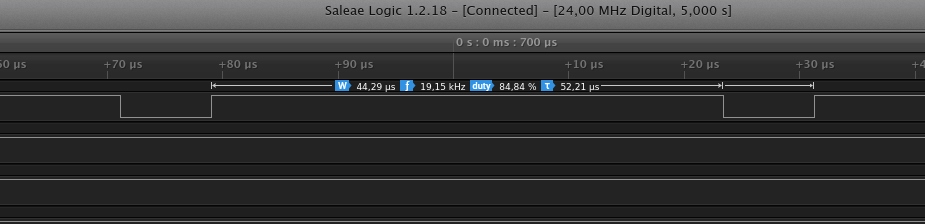
\includegraphics[width=0.85\textwidth, keepaspectratio]{imatges/ADC_LP1_Measurement.png}
 \caption{Captura de les mesures temps de l'analitzador lògic}
 \label{fig:adc_logic}
\end{figure}

\section{{\em Timers} de baix consum}
\label{sub:letimer_example}
Un mode que es fa servir sovint en sistemes de baix consum és el de tenir un {\em timer} configurat perquè desperti el sistema cada cert temps. Així per exemple, en un sistema que ha de llegir un sensor cada 30 segons, el {\em timer} seria l'únic perifèric en funcionament actiu i estaria configurat per generar una \gls{IRQ} cada 30 segons; la resta del microcontrolador podria estar en un mode de baix consum que el permeti consumir molt poca energia mentre espera a ser despertat per una \gls{IRQ}.

Al \href{https://github.com/mariusmm/cursembedded/tree/master/Simplicity/LETIMER_LP}{projecte del repositori} hi ha un exemple d'aquest tipus. Es fa servir un {\bf LETIMER}, que és un {\em timer} de baix consum i baixa freqüència que pot funcionar mentre la resta del microcontrolador està en el mode EM2 (o EM3 segons la configuració que es faci servir) \cite[294]{EFM32TGRM}. Aquest {\bf LETIMER} es pot alimentar amb el rellotge extern de baixa freqüència a 32.768 Hz ({\bf LFXO}) o bé amb l'oscil·lador intern a 1.000 Hz ({\bf ULFRCO}) (al codi es pot triar segons es defineixi o no la macro {\bf USE\_ULFRCO}). El rellotge que s'hagi triat es pre-escala per un factor suficient per tenir un comptador prou lent, ja que cal tenir en compte que aquest comptador és de només 16 bits i, per tant, si tenim una freqüència de funcionament elevada no podrem comptar gaire temps.
Tot seguit el {\em timer} es configura per generar una interrupció quan arribi a 0 (és un comptador decreixent) i el seu valor {\bf TOP} (al valor al que es reinicia després d'arribar a 0) es posa en funció de la freqüència de funcionament i el temps que es vol tenir el sistema en baix consum, a l'exemple del repositori es posa a 4 segons. Un resum del codi de l'exemple es veu a Llistat~\ref{LETIMER_example}.

\index{LETIMER0\_IRQHandler()}\index{main()}\index{LETIMER\_IntGet()}\index{LETIMER\_IntClear()}
\index{GPIO\_PinOutToggle()}\index{CMU\_ClockSelectSet()}\index{CMU\_ClockDivSet()}
\index{LETIMER\_CompareSet()}\index{EMU\_EnterEM3()}
\begin{lstlisting}[style=customc, caption={Exemple ús de {\bf LETIMER}}, label=LETIMER_example]
#define PRESCALER cmuClkDiv_1
#define EFECTIVE_CLK_FREQ (1000/PRESCALER)
#define SLEEP_SECONDS 4
#define TOP_VALUE (EFECTIVE_CLK_FREQ * SLEEP_SECONDS)

void LETIMER0_IRQHandler(void) {
	uint32_t flags;

	/* Clear flag for LETIMER0 */
	flags = LETIMER_IntGet(LETIMER0);
	LETIMER_IntClear(LETIMER0, flags);

	/* Toggle LED ON/OFF */
	GPIO_PinOutToggle(gpioPortD, 7);
}

void main(void) {
  ...
  /* ULFRCO is 1,000 kHz */
  CMU_ClockSelectSet(cmuClock_LFA, cmuSelect_ULFRCO);
  CMU_ClockDivSet(cmuClock_LETIMER0, PRESCALER);
  ...
  LETIMER_CompareSet(LETIMER0, 0, TOP_VALUE);
  ...
  while (1) {
    /* nothing to do here */
    EMU_EnterEM3(true);
  }
}
\end{lstlisting}

Aquest és un exemple senzill que fa servir un {\em timer} especial de la família EFM32 de Silicon Labs. Altres fabricants proporcionen {\em timers} similars. Així ST té un {\em timer} força similar, anomenat LPTIMER (\cite{ST_ANS4865}) i Fresscale te el LPTMR amb característiques similars \cite{Kinetis_LPTMR}. Els {\em timers} de ST i de Silicon Labs  poden generar senyals tipus \gls{PWM} mentre el microcontrolador està en modes de baix consum (veure \fullref{sub:PWM}).

\section{Baix consum i RTOS}
\label{sec:lowpwerRTOS}
Quan treballem amb un RTOS funcionant en el nostre microcontrolador, hi ha diferents estratègies per aconseguir disminuir el consum energètic.

Bàsicament hi ha dues estratègies:
\begin{itemize}
 \item Aprofitar la tasca {\em Idle} per posar al microcontrolador en un mode de baix consum.
 \item Passar a un sistema sense {\em tick} (també dit {\em tickless}).
\end{itemize}

En qualsevol cas, l'avantatge de que sigui el SO qui s'encarregui de gestionar el baix consum és que les tasques no s'han de preocupar per aquesta gestió.

\subsection{Tasca {\em Idle} per baix consum}
\label{sub:idlelowpower}
L'estratègia més senzilla és la d'activar un mode de baix consum quan s'executa la tasca {\em Idle}. Com que aquesta tasca s'executa quan no hi ha cap altra tasca preparada per agafar el microcontrolador, té sentit pensar en aturar el microcontrolador i esperar a que una tasca estigui disponible. Quan succeeixi el proper {\em tick}, el microcontrolador sortira del mode d'{\em sleep} i tornarà a executar el planificador, que, si segueix sense haver cap tasca disponible (en estat {\em Ready}) per executar tornarà a executar la tasca {\em Idle} que tornarà a adormir la CPU i es repetirà el cicle \cite{FreeRTOSLP}.

\begin{remark}
Cal recordar que quan el {\em core} està en algun mode de baix consum, el {\em SysTick} també es desactiva. Per tant, per poder tenir un {\em tick} quan el {\em core} està en un mode de baix consum caldrà fer servir un altre Timer que si que funcioni en aquests modes de baix consum.
\end{remark}

Cal pensar que tot i que aquest mètode és molt senzill d'implementar, té la limitació de que a cada {\em tick} es treu la CPU del mode de baix consum per comprovar si hi ha alguna tasca en estat {\em Ready}. Podem imaginar-nos una aplicació que llegeixi d'un sensor cada 200 ms i processant les dades, com l'aplicació d'exemple XXXXX. Si es té en compte que el {\em tick} pot ser de 1000 Hz, és fàcil d'observar que es despertarà molts cops al {\em core} perquè tant sols el planificador vegi que no hi ha cap tasca {\em Ready} i torni a adormir el processador.

%% manual break a la ultima macro pq latex no ho fa be
Aquesta característica es pot activar a FreeRTOS editant el fitxer ``FreeRTOSConfig.h'' i fixant a '0' la definició {\bf configUSE\_TICKLESS\_IDLE} i triant el valor '1' per {\bf configUSE\_SLEEP\_MODE\\\_IN\_IDLE}. En el cas de Silicon Labs, el microcontrolador es posa en el mode EM2 (veure \fullref{sec:sleepmodes}) i deixant en funcionament tant sols el RTC (veure \fullref{sub:RTC}) i les \gls{IRQ} dels GPIOs que l'usuari hagi configurat (veure \fullref{ch:IRQ}).

\subsection{FreeRTOS sense {\em tick}}
\label{sub:tickless}

L'altre estratègia per disminuir encara més el consum, és desactivar el {\em tick} durant cert temps. En una aplicació on totes les tasques estan bloquejades (i que entraria la tasca {\em Idle}) es pot calcular el temps en que alguna tasca es desbloquejarà (perquè alguna tasca estigui bloquejada perquè ha cridat la funció vTaskDelay()\index{vTaskDelay()}). Es pot desactivar el {\em Tick} i programar el Timer perquè generi una interrupció en aquell temps calculat. Si mentre està el sistema adormit esperant aquell temps hi ha algun esdeveniment extern (interrupció), es despertarà i es podrà reprendre l'execució normal i tornar a activar el {\em Tick}.

Amb aquesta estratègia es maximitza el temps en que el {\em core} està en algun dels modes de baix consum i per tant es pot reduir dràsticament el consum d'una aplicació (veure \fullref{ch:low-power}).

En el cas de FreeRTOS, el port disponible per Cortex-M ja incorpora aquesta característica, i es pot configurar editant el fitxer ``FreeRTOSConfig.h'', concretament fixant el valor '1' a la macro {\bf configUSE\_TICKLESS\_IDLE}. En el cas de Silicon Labs, el microcontrolador es posa en el mode EM2 igual que en cas amb {\em ticks} i es programa el RTC perquè generi una \gls{IRQ} en el temps adequat.

En ambdós casos el codi que gestiona el baix consum i els {\em ticks} en el port FreeRTOS està al fitxer {\bf low\_power\_tick\_management.c} a la funció {\bf vPortSetupTimerInterrupt()}\index{vPortSetupTimerInterrupt()}.

\chapter{Documentant el codi}
\label{sec:documentant}
Un tema recurrent en temes d'enginyeria del software és com documentar el codi font que es desenvolupa per tal d'afavorir, sobretot, el manteniment del codi durant el temps i algú altre (o nosaltres mateixos) haguem de modificar, re-uilitzar o arreglar algun problema. No farem aquí una discussió sobre els beneficis de documentar, quan fer-ho, etc.

Hi diferents tècniques i mètodes de documentar el codi, aquí veurem només una, basada en Doxygen. Aquest programa processa la documentació inserida dins el propi codi font i genera diferents sortides, la més habitual és una carpeta html amb tota la documentació ben bonica i accessible amb un navegador (té altres formats de sortida, com .pdf, .doc, etc.). Per documentar el nostre codi, el que cal que fem és escriure la documentació dins el propi codi com a comentaris de codi seguint unes normes i {\em tags} molt senzills propis de Doxygen. (veure Figura~\ref{fig:doxygencode}). Aquest mètode de documentar ha esdevingut un estàndard de facto i es troba arreu. Per documentar-se sobre com treballar amb Doxygen, la seva pàgina web està força bé amb exemples de tots tipus \cite{Doxygen}.

\begin{figure}
 \centering
 \fbox{\color{ocre}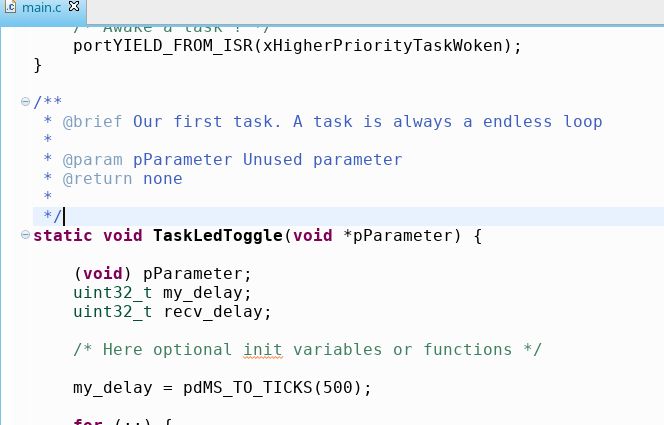
\includegraphics[width=0.85\textwidth, keepaspectratio]{imatges/Doxgen3.png}}
 \caption{Comentari per doxygen dins un codi}
 \label{fig:doxygencode}
\end{figure}

A simplicity (i de fet, a qualsevol IDE basat en Eclipse), podem activar Doxygen com l'eina de documentació, i d'aquesta manera l'editor ens ajudarà alhora d'escriure-la, ja que, per exemple, en escriure «/**» davant una funció ens inserirà automàticament el codi Doxygen per documentar-la (incloent-hi tots els paràmetres), simplificant molt la nostra feina.

Una bona opcio és afegir un directori on ficar-hi el fitxer de configuració del Doxygen (directori /Doc) i on es genera el codi html (directori /Doc/html). El Doxygen s'executa dins del directori /Doc i es genera el codi html (o pdf, o rtf, o el que calgui). Si al fitxer Doxygen li posem l'extensió .doxyfile el propi simplicity el reconeix com a fitxer de documentació i podem executar Doxygen pitjant el botó amb una arroba de color blau a la barra d'eines (Figura~\ref{fig:doxygenbutton}).

\begin{figure}[h!]
 \centering
 \fbox{\color{ocre}
\includegraphics[width=0.35\textwidth, keepaspectratio]{imatges/Doxygen_button.png}}
 \caption{Botons de Simplicity, l'arroba blava permet executar Doxygen}
 \label{fig:doxygenbutton}
\end{figure}


També podrem editar de forma visual el fitxer de configuració fent-hi doble-click i veure el resultat obrint dins del Simplicity el fitxer /Doc/html/index.html (Figura~\ref{fig:doxygenconfig}).

\begin{figure}
 \centering
 \fbox{\color{ocre}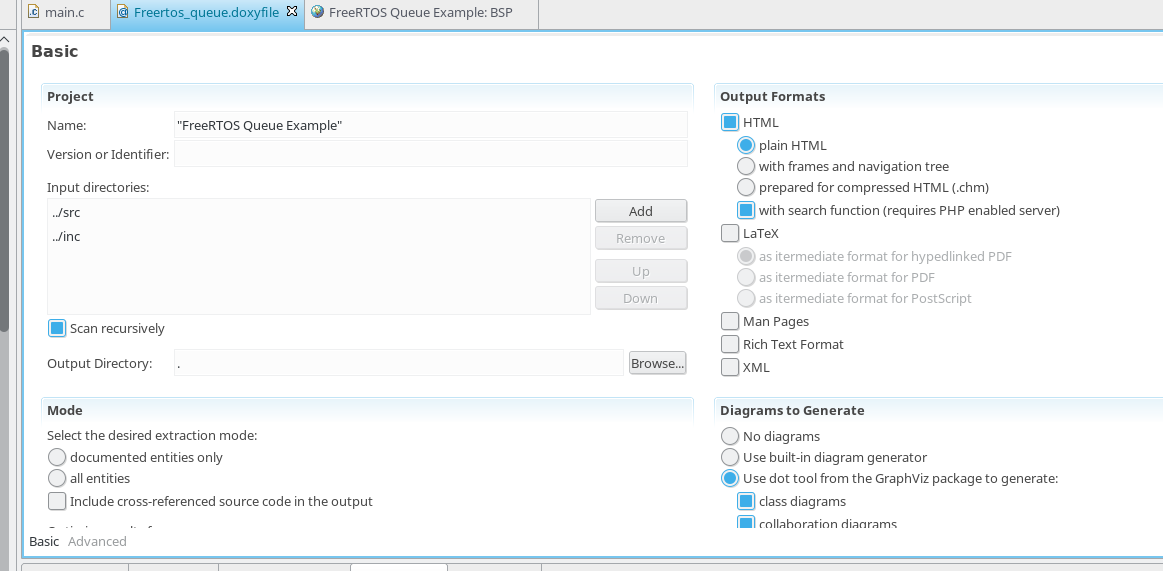
\includegraphics[width=0.85\textwidth, keepaspectratio]{imatges/Doxygent_configuration.png}}
 \caption{Configuració de Doxygen dins de Simplicity}
 \label{fig:doxygenconfig}
\end{figure}

Hi ha un exemple complet al projecte FreeRTOS Queue (veure \fullref{sub:cues_exemple}). En aquest cas, l'explicació del projecte (la secció principal anomenada mainpage en Doxygen) està al final del fitxer main.c. També hi ha la possibilitat de posar aquesta secció en un fitxer a part, normalment un fitxer README.md. Si ho fem així, aquest fitxer README.md github el presenta a la pàgina principal del projecte. El fitxer generat també es pot obrir dins el propi Simplicity Studio (Figura~\ref{fig:doxygeneclipse}).

A més, si configurem com cal github, podem pujar el codi html generat per Doxygen al repositori i veure'l a un adreça de github. La de l'exemple està a \href{https://mariusmm.github.io/cursembedded/Simplicity/FreeRTOS_1/Doc/html/}{aquí} \cite{GITHUBPages} i es pot obrir des d'un navegador qualsevol,

\begin{figure}
 \centering
 \fbox{\color{ocre}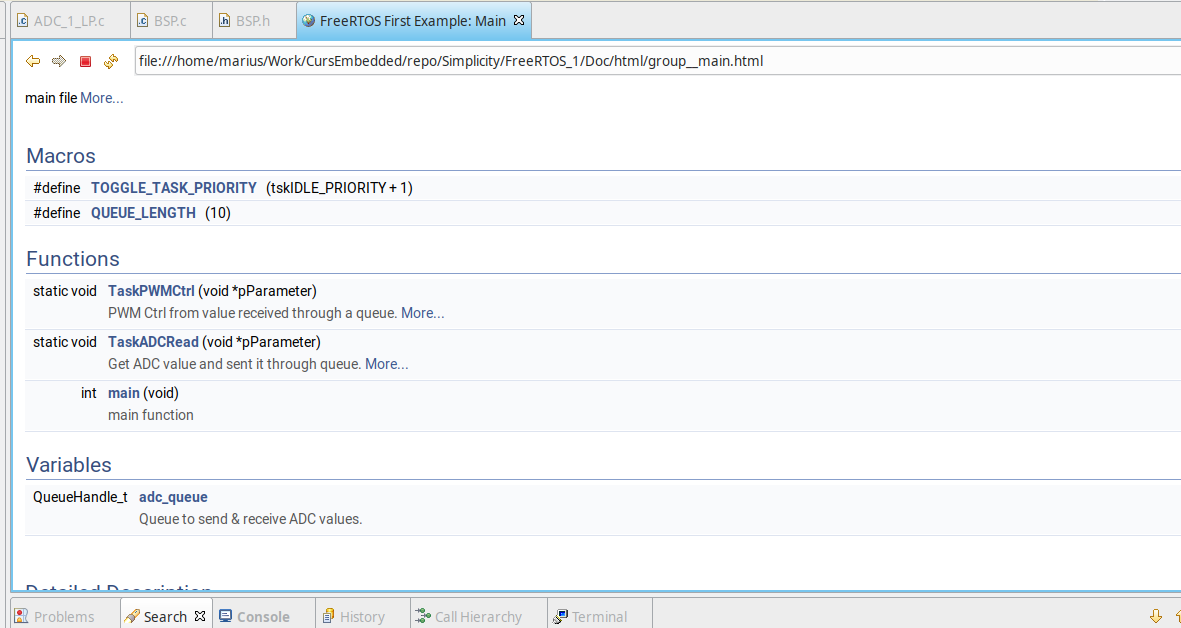
\includegraphics[width=0.85\textwidth, keepaspectratio]{imatges/DoxygenEclipse.png}}
 \caption{Pàgina web de documentació vista dins de Simplicity Studio, en aquest cas es visualitza un dels fitxers locals}
 \label{fig:doxygeneclipse}
\end{figure}

\chapter{Bones pràctiques}

En aquest capítol veurem una sèrie de bones pràctiques habituals en la programació de sistemes encastats. Aquestes bones pràctiques donen consells i guia sobre com dissenyar o programar parts de codi per evitar problemes que, habitualment, són molt complicats de detectar.
%% Veure Michael Barr Bugs1-5.pdf i Bugs6-10.pdf

\section{Ús de memòria dinàmica}
Una de les diferències més notables a l'hora d'escriure codi per un sistema encastat és l'ús de memòria dinàmica. Bàsicament se'n desaconsella totalment el seu ús en sistemes encastats. Això es deu al fet que tenim molt poca memòria RAM disponible (pocs KB) i que la possible fragmentació que s'origina en fer-ne un ús dinàmic poc exhaurir-la molt més fàcilment. A més, el fet d'usar memòria dinàmica fa que el sistema sigui menys predictible, ja que en certs casos, l'ordre en que s'executen diferents {\em malloc()} pot ser diferent a cada execució.

És per això que no s'acostuma a usar memòria dinàmica en sistemes encastats. Si, tot i la recomanació de no fer-ho, és necessari alguna mena de gestió dinàmica de la memòria, la millor opció és proveir-se d'una estructura pròpia {anomenada \em pool} de blocs d'una mida predeterminada que proporcionin aquesta funcionalitat. D'aquesta manera s'evita la fragmentació ja que tots els blocs tenen la mateixa mida.

\section{Ús de {\em volatile}}
Com ja s'ha comentat a \fullref{sb:volatile}, errors en l'ús de la paraula reservada {\em volatile} poden ocasionar {\em bugs} difícils de trobar al nostre codi. Per tant, i com a recordatori, cal definir una variable com a {\em volatile} en el següents casos:
\begin{itemize}
 \item Variable global que comunica una ISR amb una funció.
 \item Variable comptador d'un bucle per implementar un {\em delay}.
 \item Punter a una adreça de memòria corresponent a un perifèric mapat a memòria.
 \item Variable global que hi accedeixen dues o més tasques d'un RTOS.
\end{itemize}

Cal recordar que l'ús de {\em volatile} farà que les optimitzacions del compilador no s'apliquin a la variable definida com a tal.

\section{Funcions re-entrants}
Com ja es va comentar breument a \fullref{sec:wrapperI2C}, quan es treballa en un entorn multitasca (com quan es té un RTOS) cal tenir en compte que funcions que puguin ser utilitzades alhora per més d'una tasca cal que siguin re-entrants. També cal adonar-se que una biblioteca per un perifèric HW qualsevol segurament haurà de ser re-entrant, ja que diverses crides simultànies sobre el mateix HW pot ocasionar errors de funcionament.

La norma general és de protegir cada funció que hagi de ser re-entrant amb un {\em Mutex}. La funció en qüestió intentarà agafar el {\em Mutex} a l'inici de la seva execució i el retornarà en quan acabi. En el cas de biblioteques per accedir a HW, és habitual tenir un sol {\em Mutex} compartit per tota la biblioteca i que es crea quan es crida a la funció d'inicialització de la biblioteca (veure \fullref{sec:wrapperI2C}).

\section{\em Deadlock}
Un {\em Deadlock} és una situació on diverses tasques tenen una dependència circular entre elles i queden totes elles bloquejades esperant-se unes a les altres.

Per evitar aquestes situacions, sovint complexes de detectar, hi ha dues recomanacions:
\begin{itemize}
 \item Evitar adquirir dos o més {\em Mutex}. Provar d'agafar dos o més {\em Mutex} pot provocar que s'agafi un però fallin els demès, fent que la tasca hagi d'esperar a d'altres tasques els alliberin, que potser necessiten del primer {\em Mutex}.
 \item Ordenar els {\em Mutex} de manera que, si s'ha d'agafar més d'un, totes les tasques segueixin el mateix ordre.
\end{itemize}

Amb aquests dues recomanacions es poden evitar la majoria de {\em deadlocks} generats per l'ús de {\em mutex} entre tasques.

\section{Inversió de prioritats}
\label{sec:priorityinv}
Quan tenim un parell de tasques que comparteixen un recurs, una amb poca prioritat ($T_l$) i la segona amb més prioritat ($T_h$), si s'afegeix una tercera tasca amb una prioritat intermèdia ($T_m$) al sistema, podem tenir un problema d'inversió de prioritats. Això passarà quan la tasca de menys prioritat agafa el recurs compartit amb ($T_h$). En aquest moment, si la tasca de prioritat intermèdia està a l'estat {\em Ready}, passarà a executar-se, fent que la tasca ($T_l$) no s'executi i retardant l'execució de la tasca ($T_h$), fent que, de fet, la prioritat de $T_h$ i $T_m$ s'hagin invertit, ja que la tasca amb prioritat intermèdia es pot executar tot el temps que vulgui i la tasca més prioritària no té la oportunitat \cite[101]{RTEmbeddedSystems}.

La manera més senzilla de resoldre aquest problema és usar {\em Mutex} amb herència de prioritats. Aquest mecanisme fa que, provisionalment, la tasca que agafa el {\em Mutex} pugi temporalment la seva prioritat a la mateixa de la tasca que l'està esperant \cite[106]{RTEmbeddedSystems}. FreeRTOS suporta aquest mecanisme als seus {\em Mutex}, i per tant fent un bon ús dels mateixos evitarem aquest fenomen d'inversió \cite[251]{FreeRTOSBook}.

\section{Assignació de prioritats}
\label{sec:priorities_RMA}
Sovint un dels dubtes que sorgeixen en el disseny de sistemes encastats és quines prioritats cal donar a cada una de les tasques del sistema. Existeix un algorisme molt senzill per assignar les prioritats a cada tasca, basant-se en el temps de procés que necessita cada una. Aquest algorisme s'anomena {\em Rate-Monotonic Algorithm} (RMA) i fa les següents assumpcions \cite{RMA_1}\cite[136]{EmbeddedBook_2}:
\begin{itemize}
 \item Totes les tasques són periòdiques.
 \item El {\em deadline} de cada tasca és el seu període.
 \item Totes les tasques són independents.
 \item Totes les tasques són pre-emtives i el cost d'aquest és negligible.
\end{itemize}

Aquest algorisme senzillament assigna la prioritat més alta a les tasques amb un període més curt. Així, s'ordenen les tasques segons el seu període (primer els períodes més curts) i s'assignen les prioritats, de més alta a més baixa.

Per saber si es podran executar totes les tasques dins dels seus límits complint tots els {\em deadline} es poden fer els següents càlculs:

Sigui $c_i$ el temps d'execució de la tasca $T_i$. Sigui $p_i$ el període d'execució de la tasca $T_i$. Sigui $n$ el nombre de tasques totals.
Es defineix l'ús acumulat $\mu$ a:
\begin{equation*}
 \mu = \sum^{n}_{i=1}\frac{c_i}{p_i}
\end{equation*}

S'ha de complir la condició \ref{eq:RMA} perquè es compleixin tots els {\em deadlines} de totes les tasques, sempre amb els supòsits inicials.
\begin{equation}
\label{eq:RMA}
 \mu \leq n (2^{1/n}-1)
\end{equation}

\begin{table}[b]
\caption{Dades d'exemple de tasques i prioritats (temps en mil·lisegons)}
\label{tb:RMA_example}
\centering
\begin{tabular}{|c|c|c|}
\hline
{\bf Tasca} & {\bf Període $p$} & {\bf Temps d'execució $c$}\\
\hline
T1 & 500 & 20\\
\hline
T2 & 250 & 30\\
\hline
T3 & 100 & 15\\
\hline
\end{tabular}
\end{table}

Així, si tenim 3 tasques amb les dades d'execució de la Taula~\ref{tb:RMA_example} l'algorisme RMA assignarien les prioritats de la següent manera:

\begin{enumerate}
 \item T3 més prioritària.
 \item T2 prioritat intermèdia.
 \item T1 baixa prioritat.
\end{enumerate}

També es pot calcular $\mu$
\begin{equation*}
 \mu = \frac{20}{500} + \frac{30}{250} + \frac{15}{100} = 0.31
\end{equation*}
i segons l'Equació~\ref{eq:RMA} tindrem que
\begin{equation*}
 0.31 \leq n (2^{1/n}-1) = 3(2^{1/3}-1) \approx 0.78
\end{equation*}

Per tant es compleixen les condicions perquè les tres tasques es puguin executar sense perdre cap esdeveniment. L'algorisme RMA dona una conjunt de prioritats que és òptima, per tant, si no es compleixen els {\em deadlines}, cap altre mètode d'assignar prioritats fixes podrà aconseguir-ho. En aquest cas caldrà tenir un {\em scheduler} amb un algorisme de prioritats dinàmiques.

També val la pena observar que la part dreta de l'Equació~\ref{eq:RMA} té un límit:
\begin{equation*}
 \lim_{n\to\infty} n \cdot (2^{1/n}-1) = ln(2) \approx 0.7
\end{equation*}

que ens indica que amb les condicions dites abans, un sistema amb moltes tasques hauria de dedicar el 70\% d'ocupació total per garantir tots els {\em deadlines} de les tasques.

\section{Mida de les cues}
\label{sec:mida_cues}
Quan hem parlat de les cues en un \gls{RTOS} a \fullref{sec:queue}, hem dit que a l'hora de la seva creació cal especificar el tipus de dades que emmagatzemarà cada element de la mateixa i el nombre d'elements d'aquest tipus que la cua manegarà.

Però, com saber quants elements cal atorgar a una cua en la seva creació? Aquest paràmetre serà clau, ja que si creem una cua amb pocs elements disponibles, la tasca productora potser es quedi bloquejada si la tasca consumidora no va prou de pressa. Tot i que es pot triar aquest valor d'una forma empírica, començant per un valor prou baix i fent proves i via successives aproximacions arribar a un valor prou bo.

Aquest mètode, però, no ens assegura que en qualsevol cas el sistema no acabi amb una cua plena. Per això, cal un anàlisi més analític del problema per trobar una solució.

\subsection{Model M/M/1}
\label{sub:mm1}

Aquest model de cues és dels models estadístics més senzills però que ens pot donar informació important només amb les dades més bàsiques del nostre sistema. Aquest model fa certes suposicions que podem donar per bones pels nostres sistemes \cite{mm1_1}\cite{mm1_2}\cite{mm1_3}\cite{mm1_4}:
\begin{itemize}
 \item El productor genera noves entrades a la cua seguint una distribució de Poisson.
 \item El consumidor processa dades a la cua seguint una distribució exponencial.
 \item Només hi ha un productor.
 \item La cua és de tipus FIFO.
\end{itemize}

Amb aquestes suposicions ens cal trobar els paràmetres $\lambda$ i $\mu$ pel productor i el consumidor respectivament, ara es veurà com.

Si la nostra tasca consumidora genera un element nou a la cua de mitjana (seguint una distribució de Poisson) cada cert $Pr$ temps tindrem:
\begin{equation}
 Pr = \text {temps mitjà a generar una dada}
\end{equation}
i llavors tindrem que
\begin{equation}
 \lambda = \frac{1}{Pr}
\end{equation}

El mateix càlcul el podem fer pel temps de la tasca consumidora (que segueix una distribució exponencial):
\begin{equation}
C = \text {temps mitjà a processar una dada}
\end{equation}
i llavors tindrem que
\begin{equation}
 \mu = \frac{1}{C}
\end{equation}

Amb aquestes dades, tenim les següents fórmules:

\begin{equation}
 \rho = \frac{C}{Pr} = \frac{\lambda}{\mu}
\end{equation}

Aquesta primer valor $\rho$ ens indica si el sistema és factible o no: si $\rho$ és més petit d'1 ($\rho < 1$), la cua té sentit, en cas contrari, el ritme de inserir elements a la cua és més ràpid que el ritme de treure'ls i, per tant. la cua s'acabarà omplint en algun moment o altre i el productor haurà de llençar dades que no podrà inserir a la cua.

Amb aquest valor $\rho$ (o amb $Pr$ i $C$) podem obtenir els següents càlculs:

Nombre mitjà d'elements a la cua
\begin{equation}
 L_q = \frac{\rho^2}{(1-\rho)}  = \left( \frac{C}{Pr} \right)^2 /  \left( 1 - \frac{C}{Pr}\right)
\end{equation}
Temps mitjà de vida a la cua
\begin{equation}
 W_q =  \frac{\rho}{\mu - \lambda} = \frac{L_q}{\lambda} = L_q \cdot Pr
\end{equation}
Temps total d'estada en el sistema (procés més espera a la cua)
\begin{equation}
 W = W_q + \frac{1}{\mu} = W_q +C = \frac{C}{1-\rho}
\end{equation}
Nombre mitjà d'elements al sistema
\begin{equation}
 L = \frac{\rho}{(1-\rho)}  = W \cdot \lambda = \frac{W}{Pr}
\end{equation}
Probabilitat que la cua tingui més de K elements
\begin{equation}
\label{eq:Prob_queue_full}
 P(\geqslant K) = \rho^K =  \left( \frac{C}{Pr} \right)^k 
\end{equation}

Així si, per exemple, tenim una tasca productora que genera una dada cada 50 ms i una tasca consumidora que processa una dada en uns 30 ms de mitjana, tenim els següents resultats:
\begin{equation*}
Pr = 50 \text{ ms}
\end{equation*}
\begin{equation*}
C = 30 \text{ ms}
\end{equation*}
\begin{equation*}
\rho = \frac{C}{Pr} = \frac{30}{50} = 0.6
\end{equation*}
\begin{equation*}
\text{Nombre mitjà d'elements a la cua } L_q = \left(\frac{30}{50}\right)^2 / \left(1 - \frac{30}{50}\right)  = 0.9
\end{equation*}
\begin{equation*}
\text{Temps mitjà de vida a la cua } W_q = 0.9 \cdot 50 = 45 \text{ ms}
\end{equation*}
\begin{equation*}
\text{Temps total de vida d'una dada } W =  \frac{30  \cdot 50}{50-30} = 75 \text{ ms}
\end{equation*}
\begin{equation*}
\text{Nombre mitjà d'elements al sistema } L =  \frac{75}{50} = 1.5
\end{equation*}
\begin{equation*}
\text{Probabilitat que la cua tingui més de 10 elements } P(\geqslant 10) =  \left(\frac{30}{50}\right)^{10} \approx 0,00605 \rightarrow 0.60 \%
\end{equation*}

Aquestes equacions ens indiquen que durant bona part del temps de funcionament del sistema, la cua entre els dos processos tindrà tant sols 1 element, i que la probabilitat que tingui més de 10 elements en algun moment és de només el 0,60\%.
Cal fer notar que aquest valor probabilístic té en compte que els processos que generen dades es comporten com una variable aleatòria tipus Poisson i els temps de processat les dades s'ajusta a una variable aleatòria exponencial. 
Si algun dels dos processos no es comporta com a tal, si no que el seu temps de procés o de generació de dades és fix, els valors $L_q$, $W_q$, $W$ i $L$ seran certs en tot moment.

Manipulant una mica les fórmules, també podem esbrinar quin temps màxim de procés podem tenir per una tasca que genera dades cada 25 ms i volem menys d'un 0.1\% de probabilitats que la cua arribi a tenir 8 elements.

Tenim, doncs:
\begin{equation*}
 Pr = 25 \text{ ms}
\end{equation*}
\begin{equation*}
 K = 8
\end{equation*}
Segons la fórmula \ref{eq:Prob_queue_full}:
\begin{equation*}
 \text{Probabilitat que la cua tingui més de K elements} = \rho^K =  (\frac{C}{Pr})^K < 0.001 (0.1\%)
\end{equation*}

per tant tenim que
\begin{equation*}
C^8 < 25^8*0,001  \rightarrow C < \sqrt[8]{25^8 * 0,001} \approx 10.54 \text{ ms}
\end{equation*}

Això ens indica que el temps de processar una dada per part el consumidor ($C$) ha de ser menor de 10.54 mil·lisegons de mitjana per assegurar els requeriments donats.


\section{\em Debounce}
% %% SwitchDebouncing.pdf - SwitchDebouncingMore.pdf

Un problema que ens podem trobar quan volem llegir una entrada digital, és el fenomen dels rebots: si el pin està connectat a un botó a algun altre accionador mecànic aquest pot generar rebots al senyal, que vol dir que no es genera un pols quadrat i perfecte si que no quan es genera un pols aquest vagi acompanyat per d'altres polsos més petits i espuris. Habitualment les sortides d'altres components digitals no presenta aquest fenomen i no cal fer servir aquestes tècniques.

Aquest efecte pot provocar que el nostre codi compti més polsos dels que realment s'haurien de comptar i tenir un sistema erroni.

Per solucionar-ho, a part d'afegir certa circuiteria addicional al voltant del pin d'entrada, es pot desenvolupar codi que tingui en compte aquesta situació. Aquesta mena de codis es coneixen com {\em debouncing} i normalment es basen en llegir vàries vegades el pin implicat i veure quan deixa de canviar i amb això decidir si hi hagut canvi en el valor del pin o no.

Aquests algorismes han de decidir el més ràpid possible si l'entrada ha canviat o no i per contra quan més temps estiguin avaluant l'entrada millor funcionaran i detectaran espuris ({\em glitches}). A més, quan més cops per segons s'avalua el valor d'un pin més ocupació e la CPU es tindrà per aquesta tasca.

Les tècniques més habituals es basen en programar un {\em timer} o una tasca programada per que cridi una funció d'avaluació de forma periòdica (cada X mil·lisegons) i la dita funció llegeixi el valor de l'entrada i decideixi el valor real de l'entrada \cite{debounce1}\cite{debounce2}.

Un altre forma de fer-ho, potser més senzilla és la de un cop detectat un primer flanc, deixar de llegir l'entrada fins passat un temps i un cop transcorregut el temps, es llegeix el valor de l'entrada altre cop. Això es pot fer fàcilment controlant un Timer des de la ISR d'entrada del pin.

\subsection{Un exemple de {\em debouce}}
Primer cal configurar el Timer per què compti un cert temps i generi una IRQ un cop transcorregut aquest temps. Per això configurem el valor Top tal com ja vàrem fer a \fullref{sub:Timers}.

En aquest exemple es configura el valor top per que estigui comptant 100 mil·lisegons fent un càlcul molt similar al de l'exemple amb Timers anterior. També es prepara la \gls{ISR} pel {\em Timer1} tal com es veu al Llistat~\ref{timer_debouncing}

\index{TIMER1\_IRQHandler()}\index{TIMER\_IntGet()}\index{TIMER\_IntClear()}\index{GPIO\_PinInGet()}
\begin{lstlisting}[style=customc, caption=ISR del timer per fer debouncing, label=timer_debouncing]
void TIMER1_IRQHandler(void) {
  uint32_t flags;

  /* Clear flag for TIMER1 */
  flags = TIMER_IntGet(TIMER1);
  TIMER_IntClear(TIMER1, flags);

  timer_running = false;

  if (GPIO_PinInGet(gpioPortD, 8) == 1) {
    button_counter++;
  }
} 
\end{lstlisting}

La variable {\em timer\_running} es defineix com una variable booleana (i volàtil) amb valor per defecte a false. A aquesta \gls{ISR} es comprova el valor desitjat de l'entrada i si és el cas, s'actualitza el comptador.

Per últim a la ISR del \gls{GPIO} corresponent inserim el codi següent per engegar el {\em Timer} quan es detecti un flanc al senyal (un canvi al seu valor), tal com es veu al Llistat~\ref{timer_debouncing_ISR}:

\index{GPIO\_EVEN\_IRQHandler()}\index{TIMER\_TopSet()}\index{TIMER\_Enable()}
\begin{lstlisting}[style=customc, caption=Codi per engegar el timer a la ISR del GPIO, label=timer_debouncing_ISR]
void GPIO_EVEN_IRQHandler(void) {
  ...
  if (!timer_running) {
    timer_running = true;
    TIMER_TopSet(TIMER1, DEBOUNCE_VALUE);
    TIMER_Enable(TIMER1, true);
  }
...
\end{lstlisting}

D'aquesta manera tant senzilla evitarem els molests rebots i, de fet, tindrem filtrats tots els polsos que considerem massa ràpids pel nostre sistema.

\section{Ús eficient de printf}

Com ja es va veure a \fullref{sub:console_example} és possible tenir la funció {\bf printf()}\index{printf()} en els nostres sistemes encastats, pagant el preu de gastar força memòria \gls{FLASH} per la seva implementació.

Una opció recomanable en cas que l'ocupació de la memòria FLASH pugui ser un problema, és el de tenir diferents versions de {\bf printf()} segons els paràmetres que pot rebre. Així, enlloc de tenir el {\bf printf()} genèric de la biblioteca que accepta tot de tipus de tipus de dades segons el format tindrem una funció per imprimir un enter en decimal, una altra per imprimir un enter en hexadecimal, una funció per imprimir una cadena, etc. com es pot veure al Llistat~\ref{printf_variable}

A més, totes aquestes noves funciones les usarem a través d'una \gls{macro} de C, de forma que quan passem a una compilació de {\em release} del projecte aquests {\bf printf()} desapareguin del nostre codi. 

\index{printf\_char()}\index{printf\_string()}\index{printf\_hex8()}\index{printf\_int()}
\begin{lstlisting}[style=customc,caption={Diferents implementacions de {\bf printf()}},label=printf_variable]

void printf_char(char ch) {
  ITM_SendChar(ch);
}

void printf_string(char* str) {
  int i = 0;
  while(str[i]) {
    printf_char(str[i]);
    i++;
  }
}

void printf_hex8(uint8_t val) {
  if ((val >>4) > 9) {
    printf_char((val>>4) + '0' + 7);
  } else {
    printf_char((val>>4) + '0');
  }
  if ((val&0x0F) > 9) {
    printf_char((val&0x0F) +'0' + 7);
  } else {
    printf_char((val&0x0F) +'0');
  }
}

...

void printf_int(int val) {
  int rem_dec;
  int dec;
  int i;
  char buffer[10];
    
  i = 0;
    
  if (val < 0) {
    printf_char('-');
    val = -1 * val;
  }

  dec = val;
  rem_dec = val;

  do {
    rem_dec = dec%10; 
    dec /= 10; 
    buffer[i] = '0'+rem_dec;
    i++;
  } while(dec > 10);
  buffer[i] = '0' + dec;

  /* print reverse buffer */
  for(; i >= 0; i--) {
    printf_char(buffer[i]);
  }
}
\end{lstlisting}

\chapter{Empaquetant estructures}
\label{ch:estructures}

L'ús d'estructures ({\em struct} en C) per emmagatzemar dades que estan relacionades és força habitual. Per fer-ho, només cal definir una estructura i cada camp es defineix amb el tipus desitjat. Tota l'estructura funciona com un paquet de dades, que es pot moure, copiar i accedir com un tot.

Però si volem accedir a baix nivell a aquestes estructures per, per exemple, enviar les dades que conté per un port sèrie, inserir-la a un paquet de xarxa o enviar-ho a un altre dispositiu via SPI o I2C, cal que tinguem compte el problema de l'empaquetament.

Quan definim una estructura en C, el compilador ha de decidir com l'emmagatzema a la memòria. Segons les característiques dels busos i l'arquitectura del microcontrolador, pot ser que els accessos a memòria només es puguin fer a nivell de paraula (en el cas d'ARM una paraula és de 32 bits) i que no es pugui accedir a un byte individual de la memòria.

I com afecta això a les estructures? Doncs que el compilador pot optar a col·locar els diferents camps de l'estructura ocupant cada un una posició de memòria enlloc d'empaquetar-los tant com pugui.

Així, si tenim una estructura definida com es veu al Llistat~\ref{unpacket_struct} el compilador guardarà l'estructura a la memòria tal com es veu a la Figura~\ref{fig:UnpackedMemoryStructure}. 

\begin{lstlisting}[style=customc,caption={Estructura d'exemple},label=unpacket_struct]
 struct {
	uint8_t fieldS1;
	uint16_t fieldS1b;
	uint32_t fieldL1;
	uint32_t fieldL2;
	uint8_t fieldS2;
} unpacket_struct;
\end{lstlisting}


\begin{figure}
 \centering
 \fbox{\color{ocre}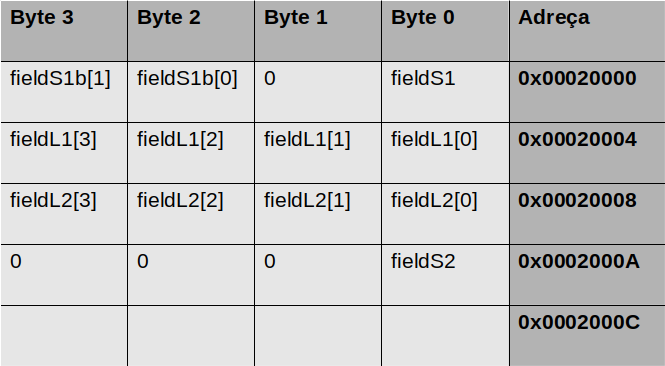
\includegraphics[width=0.85\textwidth, keepaspectratio]{imatges/Estructures.png}}
 \caption{Disposició de l'estructura a la memòria}
 \label{fig:UnpackedMemoryStructure}
\end{figure}

Que com es pot veure aquesta organització no és la que ens podríem esperar, ja que el camp {\bf fieldS1b} no està enganxat al camp {\bf fieldS1} i es per una posició de memòria per allà enmig. Aquesta operació s'anomena {\em padding} i és força habitual en totes les arquitectures. En aquest cas fa que aquesta estructura ocupi 16 bytes a la memòria enlloc dels 12 que podria ocupar si estigues tot ben empaquetat.

Això no s'acostuma a tenir gaire en compte alhora de programar sistemes encastats, però pot ser força important si en algun moment una estructura d'aquest estil cal enviar-la byte a byte a algun mòdul o perifèric. Anem a suposar que enviarem aquesta estructura d'exemple pel port sèrie. Si fem una funció que vagi llegint byte a byte l'estructura, tindrem que llegirà uns buits a 0 enmig que ens esgarraran el resultat.

En aquests casos, cal dir-li al compilador que volem que empaqueti tant com pugui l'estructura. Això és fa amb una comanda pròpia de cada compilador, en el cas de GCC és la comanda {\bf \_\_attribute\_\_} que es fa servir tal com es veu al Llistat~\ref{packet_struct}. Amb aquesta comanda l'estructura a memòria queda com es veu  a la Figura~\ref{fig:UnpackedMemoryStructure}.


\begin{lstlisting}[style=customc,caption={Estructura d'exemple empaquetada},label=packet_struct]
struct __attribute__ ((__packed__)) {
	uint8_t fieldS1;
	uint16_t fieldS1b;
	uint32_t fieldL1;
	uint32_t fieldL2;
	uint8_t fieldS2;
} packet_struct;
\end{lstlisting}


\begin{figure}
 \centering
 \fbox{\color{ocre}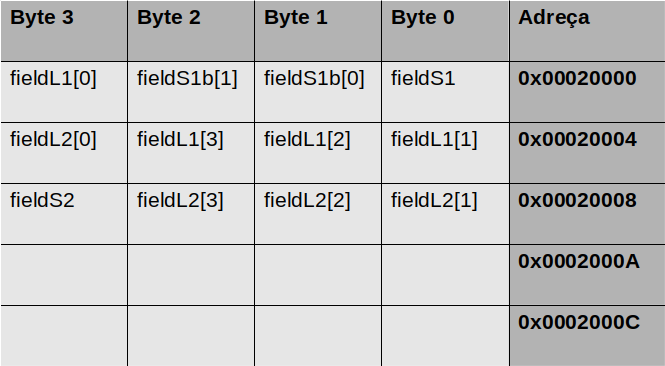
\includegraphics[width=0.85\textwidth, keepaspectratio]{imatges/Estructures2.png}}
 \caption{Disposició de l'estructura empaquetada a la memòria}
 \label{fig:UnpackedMemoryStructure}
\end{figure}

Fent servir aquest atribut es veu que està tot ben empaquetat i ens estalvia uns quants bytes. A més, s'han omplert tots els forats de manera que ara si que podrem accedir byte a byte l'estructura sense problemes.

Cal dir que en força casos aquestes estructures empaquetades poden ser més lentes d'accedir-hi, ja que la CPU haurà d'accedir a diferents posicions de memòria i reconstruir el valor original movent bits amunt i avall (veure per exemple, com es reconstruiran els camps fieldL1 o fieldL2)

\section{Un exemple senzill}

A l'\href{https://github.com/mariusmm/cursembedded/tree/master/Simplicity/Structures}{exemple del repositori} es defineixen dos estructures iguals, una amb l'atribut per empaquetar-la i l'altra amb les opcions per defecte.

Primer es treuen per la consola les mides de totes dues estructures, que encaixen amb el que hem dit aquí i tot seguit es pinten byte a byte per observar els zeros enmig i com està emmagatzemada cada estructura.

Cal destacar com s'accedeix byte a byte a l'estructura. Es defineix un apuntador a byte ({\em uint8\_t} *) i es fa apuntar a l'adreça d'inici de l'estructura que es vol analitzar. Tot seguit es va imprimint byte a byte el contingut de la memòria on està emmagatzemada l'estructura.

\begin{lstlisting}[style=customc,caption={Estructura d'exemple empaquetada},label=struct_example]
...
  uint8_t *buffer;

  buffer = (uint8_t*) &unpacket_struct;
  printf("Unpacket structure: \t");
  for(i = 0; i < sizeof(unpacket_struct); i++) {
	  printf("0x%02X, ", buffer[i]);
  }
  printf("\n");
...
\end{lstlisting}


També es pot analitzar directament el contingut de la memòria usant l'IDE Simplicity Studio fent servir l'eina de {\em dump} de la memòria tal com es veu a la Figura~\ref{fig:UnpackedMemoryStructure}.

\begin{figure}
 \centering
 \fbox{\color{ocre}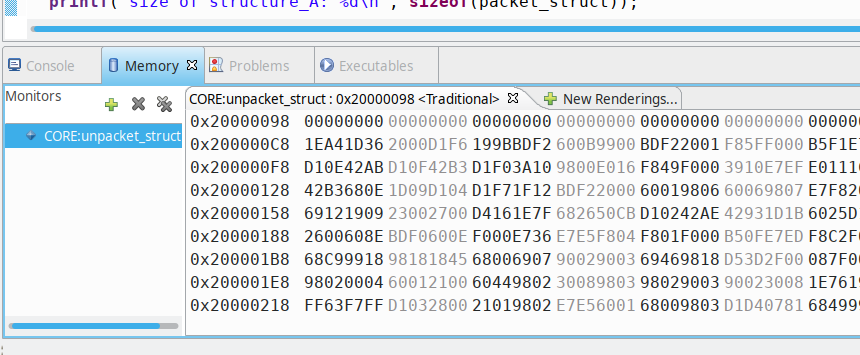
\includegraphics[width=0.85\textwidth, keepaspectratio]{imatges/MemoryDumpStructure.png}}
 \caption{Detall de la finestra de {\em memory dump} a Simplicity Studio}
 \label{fig:UnpackedMemoryStructure}
\end{figure}


\chapter{CMSIS}
\label{ch:CMSIS}
\gls{CMSIS} és una proposta d'ARM per unificar les diferents biblioteques dels fabricants sota una sola especificació, de manera que un disseny es pugui migrar a un altre fabricant de Cortex sense gaires problemes. Hi ha diferents subconjunts d'aquesta proposta, anem a veure'ls un a un.

\section{CMSIS-Core}
\label{sec:CMSIS-Core}
Aquesta part de l'especificació fixa la forma de comunicar-se amb les parts més {\em core} de la CPU, com son: el mapa de memòria (\fullref{sub:memory-mapped}), el sistema d'excepcions (\fullref{ch:exceptions}), els registres de control de la CPU, el gestor d'interrupcions (\fullref{ch:IRQ}), el Systick (\fullref{sec:systick}) i les {\em caches} \cite{CMSIS-CORE}. En aquesta biblioteca s'inclouen també els fitxers d'inicialització de cada microcontrolador en concret (\fullref{sub:boot}).

Així, i a tall d'exemple, les funcions que ja hem fet servir per controlar interrupcions com {\bf NVIC\_EnableIRQ()}\index{NVIC\_EnableIRQ()} a \fullref{ch:IRQ} no són pròpies de cap fabricant si no que són funcions definides per {\bf CMSIS-core}. També la manera en que es defineixen estructures per accedir als diferents perifèrics ve marcada per l'especificació {\bf CMSIS-Core} (veieu \fullref{devinfo}).

\section{CMSIS-Driver}
% \cite{CMSIS-DRIVER}
Aquesta especificació defineix una \gls{API} per tot un seguit de perifèrics per tal que els fabricants puguin implementar el {\em driver} corresoonent i els desenvolupadors no hagin de dependre de llibreries pròpies de cada fabricant. Aquesta especificació inclou els següents perifèrics:
\begin{itemize}
 \item \gls{CAN}
 \item Ethernet
 \item I2C
 \item \gls{MCI}
 \item  NAND 
 \item Flash
 \item \gls{SAI}
 \item SPI
 \item Storage
 \item USART
 \item USB
\end{itemize}


\section{CMSIS-DSP}
\label{sec:CMSIS-DSP}
Aquesta biblioteca inclou totes les funcions específiques de tipus \gls{DSP} dels Cortex-M més avançats (Cortex-M4 i Cortex-M7) i funcions que treballen amb punt flotant per tot tipus de Cortex-M. Si el Cortex-M amb el que treballem suporta punt flotant, la biblioteca farà les operacions per HW, i les farà per SW en cas contrari \cite{CMSIS-DSP}\cite{AN0051}.

\section{CMSIS-RTOS}
\label{sec:CMSIS-RTOS}
Aquesta biblioteca defineix un conjunt de funcions i crides per ``amagar'' el sistema operatiu que es pugui fer servir, de manera que es pugui intercanviar el \gls{RTOS} sense afectar al codi d'aplicació \cite{CMSIS-RTOS}.

D'aquesta manera es tenen crides estàndard per les funcions habituals (crear tasques, semàfors, cues, etc., enviar dades a la cua, etc.) i així es pot, en principi, intercanviar el RTOS sense haver de canviar res del codi d'usuari. Fent servir aquesta API no cal conèixer les interioritats i particularitats de cada RTOS que es vulgui fer servir, ja que quedaran amagades i pre-configurades per la biblioteca.

Així tenim que ST proporciona un \gls{wrapper} de CMSIS-RTOS per FreeRTOS que s'integra fàcilment al seu IDE \cite{ST-CMSIS-RTOS}. Silicon Labs no proporciona suport per aquesta biblioteca, però es pot fer servir el \gls{wrapper} de codi obert disponible a \href{https://github.com/labapart/polymcu/tree/master/RTOS/FreeRTOS/cmsis}{GitHub}.

A part, es va crear una implementació de CMSIS-RTOS anomenada CMSIS-RTOS-RTX (o també Keil RTX) per part de Keil (empresa propietat d'ARM) \cite{Keil-RTX}.

\section{CMSIS-DAP}
\label{sec:CMSIS-DAP}
Més que una biblioteca, aquesta part de CMSIS és una definició de com ha de treballar un dispositiu que faci de pont entre un port USB i el port de configuració dels microcontroladors Cortex. Això possibilita que, per exemple, la placa de prototipat tingui un port USB i el puguem fer servir per programar el microcontrolador, tenir la consola de {\em debug} (SWO), poder inspeccionar registres de la CPU, etc. \cite{CMSIS-DAP}.

\section{CMSIS-NN}
\label{sec:CMSIS-NN}
Aquesta biblioteca està composta d'un seguit de funcions i algorismes per implementar xarxes neurals a processadors Cortex-M i queda fora de l'objectiu d'aquest llibre \cite{CMSIS_NN_paper}\cite{CMSIS-NN}.

\chapter{Normes de codificació}
\label{sec:GuiesProgramacio}

Per tal d'unificar estils de codi i per evitar possibles errors, és habitual seguir algun conjunt de normes de codificació quan es desenvolupa un projecte. Aquest costum de normes acostumen a ser una llista de recomanacions d'estil sobre l'escriptura del codi, normes sobre coses prohibides o no recomanades, etc, Per cara regla, s'acostuma a donar una breu explicació del motiu. Aquests conjunts de normes acostumen a ajudar a evitar {\em bugs} de difícil detecció.

\begin{remark}
Tot i que un conjunt de normes de codificació ajuda a no inserir {\em bugs}, les normes per si soles no poden garantir que no es generin {\em bugs} en un sistema complex. Cal sempre seguir les bones pràctiques de Test.% (veure \fullref{part:test}).
\end{remark}

Normes generals n'hi ha moltes i alguna de les mes populars és la coneguda com ``The Power of 10: Rules for Developing Safety-Critical Code'' (``El poder del 10: regles per desenvolupar codi crític'' \cite{powerof10}. En aquest document es presenten tant sols només 10 regles per ajudar a escriure codi més segur i menys propens a errors. 

En àmbits molt específics hi ha normes i estàndards propis, com el DO-178 per l'àmbit aeri i espacial; IEC 61508, ISO 26262 o SAE J3061 per automoció o IEC 62304 per l'industria mèdica. Per l'àmbit espacial el JPL ({\em Jet Propulsion Laboratory}) té publicada una norma pròpia \cite{JPLCProgramming}.

També hi ha normes genèriques, que no es centren a cap àmbit concret. Les normes genèriques més habituals i conegudes són MISRA-C \cite{MISRAHomepage} i ``Embedded C Coding Standard'' \cite{BARRGuidelines}. Per espai, la \gls{ESA} fa servir el document  ``C and C++ Coding Standards'' \cite{BSSC}.

Es descriuen breument als apartats següents.

\section{\em The Power of 10: Rules for Developing Safety-Critical Code}
Aquest conjunt de només 10 regles es va escriure per ajudar a l'anàlisi estàtic del codi i la revisió per desenvolupadors. Es poden resumir en:
\begin{itemize}
 \item Evitar construccions complexes com {\em goto} i l'ús de recursivitat.
 \item Tots els bucles han de tenir fitada la seva longitud.
 \item Evitar l'ús de memòria dinàmica.
 \item Restringir la llargada d'una funció a 60 línies.
 \item Fer servir un mínim de dos comprovacions en temps d'execució per cada funció.
 \item Restringir la vida de les dades el més possible.
 \item Comprovar el valor de retorn de totes les funcions que retornen un valor.
 \item Poc ús del pre-processador.
 \item Limitar l'ús de punters a una sola indirecció i no usar punters a funcions.
 \item Compilar amb tots els {\em warnings} activats. Resoldre sempre tots els {\em warnings} abans de publicar el codi.
\end{itemize}


\section{MISRA-C}
\label{sec:MISRA}
MISRA C és un conjunt de normes i guies per programar en codi C per sistemes encastats. Es va proposar per primer cop el 1997 per l'associació MISRA (sigles de {\em Motor Industry Software Reliability Association}) i ha tingut diverses revisions, la tercera i última es va publicar el 2012 \cite{MISRAHomepage}\cite{MISRAC2012}.
Aquestes especificacions cal comprar-les (la versió digital costa 15 lliures) i no es poden redistribuir lliurement, però si podem tenir accés a algun addenda per veure com són aquestes normes \cite{MISRAAmend}.

Aquestes normes es divideixen en 3 classificacions segons el grau d'obligatorietat:
\begin{itemize}
 \item {\em Mandatory} són normes que s'han de complir sense cap excepció
 \item {\em Required} són normes a complir però es poden incomplir si hi ha una explicació racional (anomenada {\em Deviations}
 \item {\em Advisory} que són normes optatives, però no cal complir-les, tot i que es recomana fer-ho.
\end{itemize}

Les normes consten d'una frase dient què s'ha de fer o no s'ha de fer, una explicació del perquè de la norma i un exemple de l'ús correcte.

Així si mirem a l'addenda 1 \cite[4]{MISRAAmend} (que és de lliure distribució i accés), la regla 21.14 diu que la funció {\bf memcmp()}\index{memcmp()} no s'ha de fer servir en altre cosa que no siguin cadenes acabades en NULL ('\textbackslash 0'). Aquesta norma evita que es puguin fer servir {\em buffers} d'una mida superior a la cadena de text que guarden i provoqui errors que poden ser molt complexes de trobar.

Existixen eines que automàticament comproven la conformitat d'un projecte o codi a les normes MISRA. Entre aquestes eines, algun compilador fa la comprovació en temps de compilació (ho fan els compiladors d'IAR i de TI).

Per últim, cal dir que hi ha força controvèrsia amb d'idoneïtat de seguir les normes MISRA, donat les limitacions que provoca al desenvolupador i les suposades avantatges que proporciona.

\section{\em Embedded C Coding Standard}
Aquestes normes són de lliure accés i escrites pel Barr Group. Conté regles tant d'estil de text (número de caràcters per línia, on posar els '\{', etc.) com regles de sintaxi en C, com per exemple quan i on usar la paraula reservada {\em volatile}, etc. Segons el mateix document, aquestes regles són més laxes que les normes MISRA \cite{BARRGuidelines}.

En aquest cas, cada regla consta de l'explicació de la regla en si mateixa, el raonament que hi ha per definir la regla, quan pot haver-hi una excepció i com aplicar-la.

També hi ha eines per comprovar que el codi escrit segueix aquestes normes.

\section{\em JPL Institutional Coding Standard for the C Programming Language}
Aquesta normes de codificació venen d'un laboratori del JPL per tal d'aconseguir millor seguretat i qualitat en el software que s'escriu a les sondes espacials d'aquesta institució \cite{JPLLARS}.

Les normes de codificació son una ampliació de les normes MISRA per afegir-hi sistemes multi-tasca \cite{JPLCProgramming}. Es defineixen nivells d'acompliment amb les normes, anant des de LOC-1 fins a LOC-4 amb un total de 120 regles. La majoria de regles son equivalents a algunes de les normes MISRA. Els dos últims nivells d'acompliment (LOC-5 i LOC-6) consisteixen a acomplir amb totes les regles obligatòries o opcionals de les normes MISRA.

Així, com a diferència de regles que es poden trobar a d'altres normes de codificació, aquestes afegeixen regles com la Regla 6, que demana que sempre es facin servir mecanismes IPC per comunicar tasques entre si, i que cap tasca ha d'accedir a dades o executar codi d'altres tasques. La Regla 7 demana que les tasques no se sincronitzin fent servir {\em delay}.

\chapter{DSP}
\label{ch:DSP}
Com ja s'ha comentat, els Cortex-M4 i Cortex-M7 suporten instruccions addicionals de tipus \gls{DSP} \cite[173]{GuideCortexM3M4}\cite[255]{DesignersGuide}:
\begin{itemize}
 \item Instruccions tipus \gls{SIMD}
 \item Instruccions de saturació
 \item Instruccions addicionals de multiplicació i \gls{MAC}
 \item Instruccions de empaquetar i desempaquetar
 \item Opcionalment, instruccions de punt flotant
\end{itemize}

Aquestes instruccions s'afegeixen al conjunt d'instruccions màquina de la CPU i permeten que els processadors Cortex-M puguin implementar algorismes de DSP de forma prou eficient. Com que moltes d'aquestes instruccions i nous tipus de dades no són estàndard dins els compiladors de C més habituals, \gls{ARM} proporciona la biblioteca CMSIS-DSP (veure \fullref{sec:CMSIS-DSP}). Aquesta biblioteca, curiosament, es pot fer servir tant en Cortex-M4 i M7, com en Cortex-M3 i M0 que no tenen instruccions específiques de DSP.

Per fer-la servir cal fer, almenys, dues passes:
\begin{enumerate}
 \item Definir un símbol de compilació segons el processador amb el que estiguem treballant ({\bf ARM\_MATH\_CM0}, {\bf ARM\_MATH\_CM3}, {\bf ARM\_MATH\_CM4}).
 \item Afegir la biblioteca pre-compilada al nostre projecte (er això cal afegir també el {\bf PATH} on està situada la biblioteca) tal com es veu a la Figura~\ref{fig:EnableDSP}.
\end{enumerate}

\begin{figure}
 \centering
 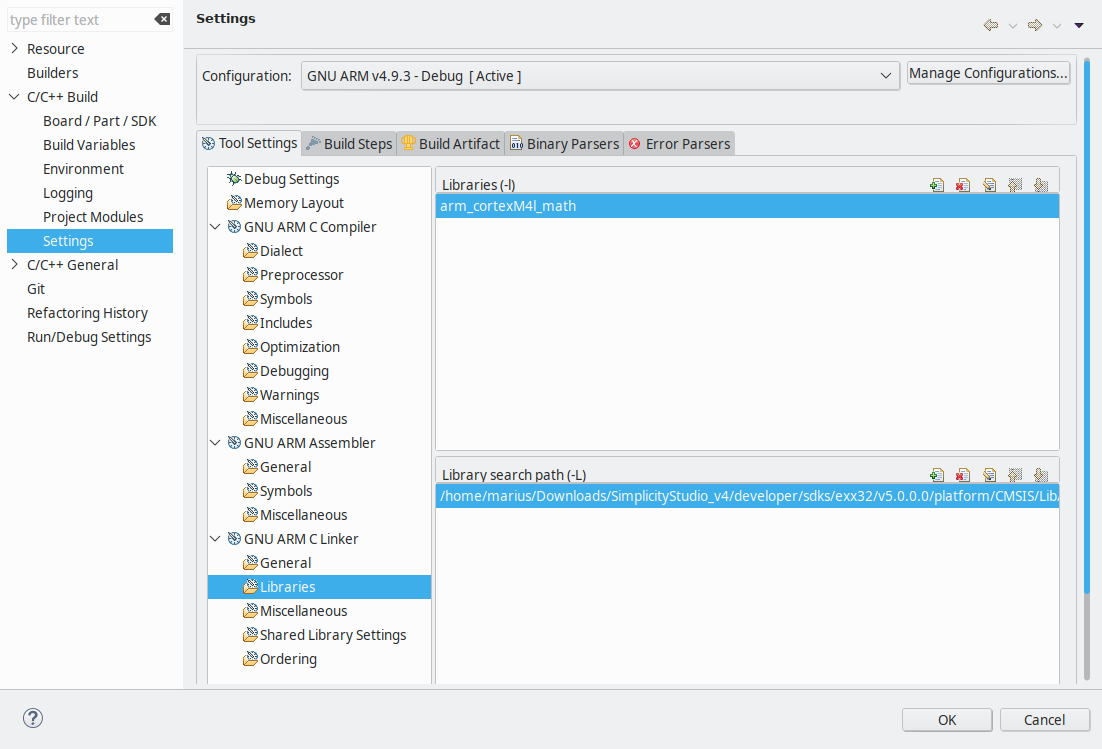
\includegraphics[width=0.85\textwidth, keepaspectratio]{imatges/EnablingDSP_Lib.png}
 \caption{Configuració del Simplicity Studio afegint-hi la biblioteca CMSIS-DSP}
 \label{fig:EnableDSP}
\end{figure}

La documentació de la biblioteca proporciona totes les funcions implementades així com un conjunt d'exemples dels usos més comuns \cite{CORE-DSP}. SiliconLabs també proporciona documentació en un {\em Application Note} sobre la biblioteca \cite{AN0051}.

\chapter{C++ vs C}
\label{ch:CvsCPP}
En aquest llibre s'ha treballat exclusivament en llenguatge C (versió C99) i no s'ha parlat res de C++. Anem a fer-ho ara en aquest capítol.

La discussió sobre usar o no C++ en sistemes encastats deu ser tant antiga com l'aparició d'aquest llenguatge orientat a objectes. Si bé als seus inicis el llenguatge presentava força problemes, ja fa molts anys que és un llenguatge estable i candidat a ser usat en sistemes encastats. Tot i això, la seva popularitat ha estat desigual i encara hi ha molts equips de desenvolupadors de sistemes encastats que treballen exclusivament en C.

Els problemes habituals que s'ha acusat al C++ per no fer-lo servir en sistemes encastats són els següents \cite{CXX_1}:
\begin{itemize}
 \item codi més llarg: si bé això pot ser veritat, les mides de les memòries \gls{FLASH} dels microcontroladors és cada cop més gran i els compiladors moderns generen codi força optimitzat, a més que es poden desactivar opcions del llenguatge que no es fan servir.
 \item més lent: això era cert amb els primers compiladors de C++, però actualment el codi generat és de la mateixa qualitat que el generat pels compiladors de C.
 \item més {\em stack}: seguint les mateixes normes que amb C, és possible tenir codi C++ que faci un ús correcte de l'{\em stack}
\end{itemize}

En canvi, els avantatges que ens pot proporcionar treballar amb C++ poden ser:
\begin{itemize}
 \item comprovació de tipus en temps de compilació. C és força laxe en aquest tema, i això pot conduir a errors. C++ és capaç de fer comprovacions en temps de compilació per avaluar la correcció de les conversions.
 \item {\em namespaces}, que permeten classificar i organitzar el codi d'una forma intuïtiva i senzilla.
 \item constructors i destructors permeten inicialitzar i destruir o netejar estructures de forma automàtica.
 \item orientació a objectes, l'organització del codi en objectes pot ajudar a ordenar i simplificar el codi.
 \item sobrecàrrega d'operadors, fent que operacions entre objectes sigui senzilla amb un codi resultant força senzill.
\end{itemize}

També cal recordar que no cal fer servir totes les noves capacitats de C++ respecte a C de cop, si no que es poden anar incorporant poc a poc al nostre codi conforme anem guanyant experiència i coneixements.

Dues de les característiques de C++ que ocupen força memòria són el \gls{RTTI} i el control d'excepcions. RTTI dona informació del tipus de classes polimòrfiques (que tenen almenys un mètode virtual) i és una característica que es faci servir gaire en sistemes encastats. El control d'excepcions permet l'execució d'un mètode i capturar l'error que es pugui generar i tractar-lo fora de la funció i de forma controlada.

Aquestes dues característiques de C++ afegeixen força codi a qualsevol projecte amb el que treballem, fent que, per exemple, no puguem compilar un simple ``Hello World embedded'' per la nostra placa de desenvolupament ja que ocupa massa FLASH. Les opcions per deshabilitar aquestes funcions al compilador GNU (que és el compilador utilitza Simplicity Studio) son:
\begin{verbatim}
-fno-rtti -fno-exceptions
\end{verbatim}

\begin{figure}
 \centering
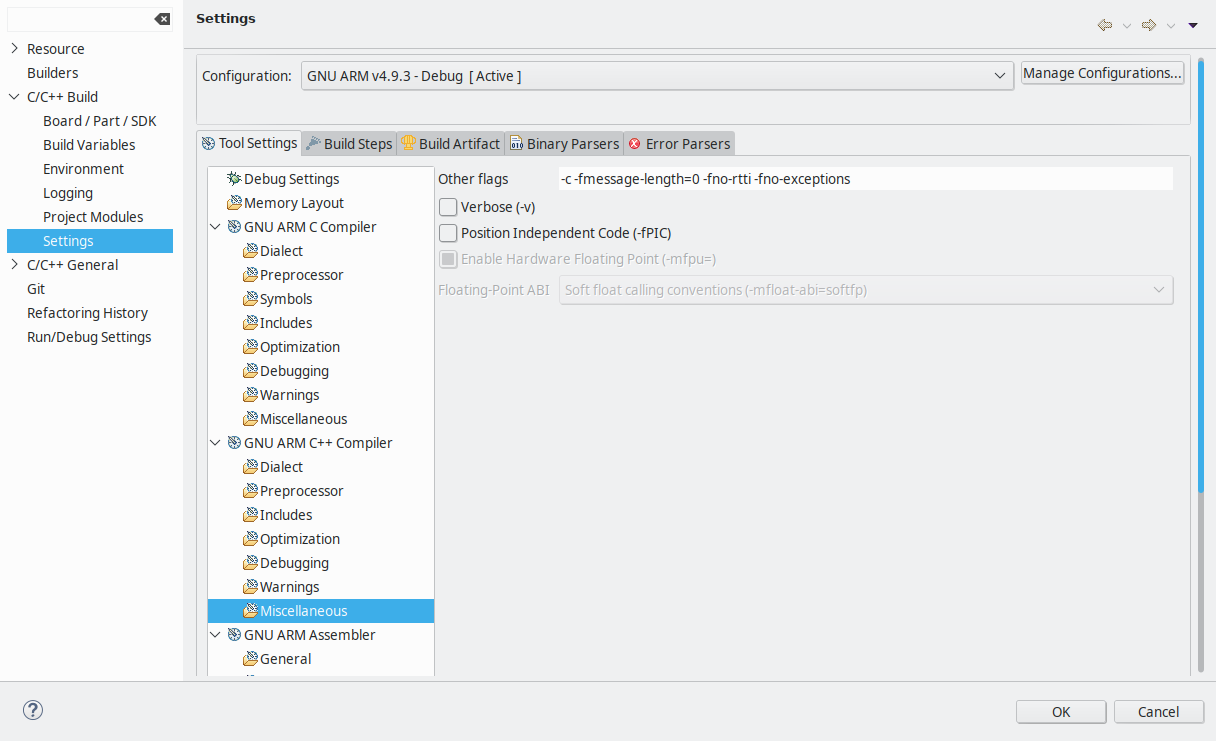
\includegraphics[width=0.85\textwidth, keepaspectratio]{imatges/CXX_options.png}
 \caption{Configuració Simplicity Studio per deshabilitar RTTI i les excepcions}
 \label{fig:CXX_RTT}
\end{figure}
i es configura tal com es veu a la Figura~\ref{fig:CXX_RTT}.

\section{Primer exemple en C++}
\label{sec:CXX_example}
\href{https://github.com/mariusmm/cursembedded/tree/master/Simplicity/CXX_1}{L'exemple CXX\_1} és el típic ``Hello World'' per sistemes encastats escrit en C++.

Aquest exemple fa servir dues classes dins el {\em namespace} {\bf BSP}.

\subsection{LED}
Com el seu nom indica, serveix per controlar l'únic \gls{LED} de la \gls{PCB} de prototipat. Està basada en una classe amb tres mètodes senzills per controlar un sol LED (LED::On(), LED::Off(), LED::Toggle())\index{LED::On()}\index{LED::Off()}\index{LED::Toggle()}.
Dins el constructor s'activa el rellotge pel perifèric \gls{GPIO} i es configura el pin corresponent al LED de la PCB (Llistat~\ref{LED_class}).

 \begin{lstlisting}[caption={Part del codi de la classe LED},style=customc,label=LED_class]
LED::LED() {
  CMU_ClockEnable(cmuClock_GPIO, true);
  GPIO_PinModeSet(gpioPortD, 7, gpioModePushPullDrive, 0); /* LED */
}
...
void LED::On() {
  GPIO_PinOutSet(gpioPortD, 7);
}
\end{lstlisting}


\subsection{Button}
Aquesta classe gestiona el valor d'una entrada del \gls{GPIO} d'una fora senzilla, la classe {\bf Button} emmagatzema els paràmetres d'un pin d'E/S i abstreu les crides a la biblioteca {\bf emlib} de Silicon Labs (veure Llistat~\ref{Button_class}).

\begin{lstlisting}[caption={Part del codi de la classe LED},style=customc,label=Button_class]
Button::Button(GPIO_Port_TypeDef port, int pin, bool pull, bool pullup) {

  CMU_ClockEnable(cmuClock_GPIO, true);

  m_port = port;
  m_pin = pin;
  m_pull = pull;
  m_pullup = pullup;

  if (m_pull == false) {
    GPIO_PinModeSet(port, pin, gpioModeInput, 0);
  } else {
    if (m_pullup == true) {
      GPIO_PinModeSet(port, pin, gpioModeInputPull, 1);
    } else {
      GPIO_PinModeSet(port, pin, gpioModeInputPull, 0);
    }
  }
}

bool Button::getValue() {
  unsigned int pin_value;

  pin_value = GPIO_PinInGet(m_port, m_pin);
  if (pin_value == 0) {
    return false;
  } else {
    return true;
  }
}
\end{lstlisting}

\subsection{Un {\em Hello World} ``més C++''}
A continuació modifiquem l'exemple per donar-li una volta més i que sigui més ``estil C++'' (està al \href{https://github.com/mariusmm/cursembedded/tree/master/Simplicity/CXX_2}{repositori}). El que s'ha fet ha estat crear una nova classe {\bf Pin} que abstrau la informació d'un pin GPIO d'EFM32. La classe {\bf Button} fa servir {\bf Pin} per obtenir les característiques del GPIO a controlar.

\subsection{Mida dels executables}
\label{CXX_size}
A \href{https://github.com/mariusmm/cursembedded/tree/master/Simplicity/CXX_1}{l'exemple CXX\_1} tenim el ``Hello World embedded'' fet en C++ de manera bàsica. A \href{https://github.com/mariusmm/cursembedded/tree/master/Simplicity/CXX_2}{l'exemple CXX\_2} s'ha fet una implementació ``més C++'' amb la mateixa funcionalitat. A la Taula~\ref{tb:CXX_size} es pot veure la quantitat de memòria de tot tipus que necessiten les dues aplicacions així com l'exemple bàsic en C.

\begin{table}[!htbp]
\caption{Ocupació de memòria de ``Hello World embedded '' en C i C++ (tots els projectes compilats amb optimització -O2).}
\centering
\begin{tabular}{|c|c|c|c|}
\hline
{\bf Aplicació} & {\bf text} & {\bf data} & {\bf bss}\\
\hline
{\bf GPIO\_1} & 972 & 108 & 28 \\
\hline
{\bf CXX\_1} & 1836 & 112 & 32 \\
\hline
{\bf CXX\_2} & 2076 & 112 & 32 \\
\hline
\end{tabular}
\label{tb:CXX_size}
\end{table}

Com a curiositat, l'ús de {\em std::cout} de la biblioteca {\em iostream} i l'operador {\bf <{}<} afegeix uns 150KB de codi FLASH (!!!), fent que sigui poc recomanable o impossible de fer servir en un sistema encastat actual.

\section{Un {\em driver} en C++}
Com hem vist al llarg del llibre, bona part del codi són {\em drivers} per controlar els diferents perifèrics o dispositius del nostre sistema encastat. Si treballem en C++, caldrà que aquest {\em drivers} els fem també en C++. Veurem ara un exemple amb la \gls{UART}, escrivint un {\em driver} i un exemple igual al vist a \fullref{sec:UART_example_2}.

En \href{https://github.com/mariusmm/cursembedded/tree/master/Simplicity/CXX_UART}{aquest exemple} tenim una classe \gls{UART} que és la implementació del {\em driver} per la UART que es va veure a l'exemple de la Secció \ref{sec:UART_example_2}. Aquesta classe {\bf UART}\index{UART class} fa servir {\em buffers} circulars per emmagatzemar les dades que es reben o s'han d'enviar per la UART i té els mètodes {\bf AvailableData()}, {\bf GetData()} i {\bf SendData()}\index{UART::AvailableData()}\index{UART::GetData()}\index{UART::SendData()} com ja tenia el mòdul UART de l'exemple en C. Aquests mètodes tant sols accedeixen al {\em buffer} circular adequat (de transmissió o recepció) que està implementat a la classe {\bf CircularBuffer} \index{CircularBuffer class}.

Tal com es veu al Llistat~\ref{operator_UARTCXX} s'ha sobrecarregat l'operador {\bf<{}<} per fer més fàcil l'ús de la classe a l'hora d'enviar dades i poder escriure codi com el del Llistat~\ref{operator_UARTCXX_example}.

\index{UART::<{}<}
\begin{lstlisting}[style=customc,caption=Ús de l'operador <{}< de la classe UART,label=operator_UARTCXX_example]
  my_uart << "Testing" << " C++ string style";
\end{lstlisting}


\index{UART::<{}<}\index{UART class}\index{UART::Tx()}
\begin{lstlisting}[style=customc,caption=Implementació de l'operador <{}< per la classe UART,label=operator_UARTCXX]
class UART {
  ...
  UART& operator<<(char* str) {
    for(char* it = str; *it; ++it) {
      this->Tx(*it);
    }
    return *this;
  }

  UART& operator<<(std::string str) {
    for(std::string::iterator it = str.begin(); it != str.end(); ++it) {
      this->Tx(*it);
    }
    return *this;
  }
  ...

  void UART::Tx(unsigned char c) const {
    USART_Tx(m_uart, c);
  }
  ...
}

\end{lstlisting}

La resta del codi és prou autoexplicatiu a excepció de l'implementació de les \glspl{ISR} de la UART. En aquest cas ens trobem que les \glspl{ISR} haurien d'estar encapsulades dins la pròpia classe UART\index{UART class} però això no és possible, donat que la classe no és estàtica, i per tant ``no existeix'' fins que no es crea instanciant un objecte d'aquest tipus \cite{ISRCXX}\cite{ISRCXX_2}. Una possible solució a aquest problema és el que es veu al codi~\ref{ISR_UARTCXX}: es té el codi pròpiament dit de la \gls{ISR} a uns mètodes privats de la classe del {\em driver} (en aquest cas la classe UART) i en algun altre lloc del codi (en aquest exemple al fitxer {\em main}\index{main()}) s'insereix la construcció que es veu al Llistat~\ref{main_ISR_UARTCXX}. D'aquesta manera les \glspl{ISR} criden als mètodes adequats de la classe pertinent.

\index{UART::USART1\_TX\_IRQHandler()}\index{UART::USART1\_RX\_IRQHandler()}\index{UART class}
\begin{lstlisting}[style=customc,caption=Implementació de les ISRs en C++,label=ISR_UARTCXX]
void UART::USART1_TX_IRQHandler(void) {
  USART_IntClear( USART1, USART_IEN_TXC);
  Send();
}

void UART::USART1_RX_IRQHandler(void) {
  char data;

  if (USART1->IF & LEUART_IF_RXDATAV) {
    data = USART_Rx(USART1);
    m_RX.PushData(data);
    USART_IntClear( USART1, USART_IEN_RXDATAV);
  }
}

class UART {
  ...
  friend void USART1_TX_IRQHandler();
  friend void USART1_RX_IRQHandler();

private:
  void USART1_TX_IRQHandler(void);
  void USART1_RX_IRQHandler(void);
  ...
}
\end{lstlisting}

\index{USART1\_TX\_IRQHandler()}\index{USART1\_RX\_IRQHandler()}\index{UART class}
\begin{lstlisting}[style=customc,caption=Part del fitxer UART.cpp de l'exemple d'us del {\em driver} en C++ per la UART,label=main_ISR_UARTCXX]
static UART* helper_uart;

void USART1_TX_IRQHandler() {
  helper_uart->USART1_TX_IRQHandler();
}

void USART1_RX_IRQHandler() {
  helper_uart->USART1_RX_IRQHandler();
}
\end{lstlisting}

\subsection{Ocupació de memòria}
De nou, anem a analitzar l'espai de memòria necessari per aquest exemple comparat amb l'exemple escrit en C amb la mateixa funcionalitat.

El codi en C++ es compila amb 3 variants:
\index{UART::<{}<}
\begin{itemize}
 \item Sobrecarregant l'operador {\bf <{}<} que pugui rebre dades de tipus {\em char}.
 \item Sobrecarregant l'operador {\bf <{}<} que pugui rebre dades de tipus {\em std::string}.
 \item Sense sobrecarregar l'operador.
\end{itemize}

Els resultats es mostren a la Taula~\ref{tb:UAR_CXX_size_O2}. Es pot veure que l'ús de l'operador que suporta {\em std::string} afegeix força codi ROM (segona columna a la Taula, uns 2 KB) i que, en general, l'ús de C++ afegeix un sobrecost en espai ROM al nostre codi. Potser el més destacable és que la quantitat de RAM necessària no s'incrementa de manera significativa, sent aquest recurs el més escàs en un microcontrolador.

% \begin{table}[!htbp]
% \caption{Ocupació de memòria d'exemple amb la UART en C i C++ (tots els projectes compilats sense optimització -O0).}
% \centering
% \begin{tabular}{|c|c|c|c|}
% \hline
% {\bf Aplicació} & {\bf text} & {\bf data} & {\bf bss}\\
% \hline
% {\bf Sense operador <{}<} & 5436 & 120 & 40 \\
% \hline
% {\bf Amb operador <{}< i char} & 5452 & 120 & 40 \\
% \hline
% {\bf Amb operador <{}< i std::string} & 7812 & 128 & 168 \\
% \hline
% {\bf Original C} & 4424 & 116 & 184\\
% \hline
% \end{tabular}
% \label{tb:UAR_CXX_size_O0}
% \end{table}

\begin{table}[!htbp]
\caption{Ocupació de memòria d'exemple amb la UART en C i C++ (tots els projectes compilats amb optimització -O2, en KB).}
\centering
\begin{tabular}{|l|c|c|c|}
\hline
{\bf Aplicació} & {\bf text} & {\bf data} & {\bf bss}\\
\hline
{\bf Sense operador <{}<} & 4636 & 120 & 40 \\
\hline
{\bf Amb operador <{}< i char} & 4644 & 120 & 40 \\
\hline
{\bf Amb operador <{}< i std::string} & 6796 & 128 & 168 \\
\hline
{\bf Original en C} & 2620 & 116 & 184\\
\hline
\end{tabular}
\label{tb:UAR_CXX_size_O2}
\end{table}





\section{Conclusions}
Tot i que l'ús de C++ enlloc de C incrementa la mida de l'executable final i les seves necessitats de memòria, el seu ús pot estar justificat en casos on l'encapsulació que proporciona C++ ajudi a la claredat del codi o a la portabilitat del mateix a diferents plataformes.

En qualsevol cas, cal una expertesa en el llenguatge per fer-ne un bon ús per tenir en compte les particularitats d'escriure codi C++ per sistemes encastats.


\chapter{Relació Esquemàtic i FW}
\label{ch:schematic}
Quan es dissenya un sistema encastat, una de les parts més importants i on contribueixen perfils professionals de diferent mena és la del disseny de l'esquemàtic. Aquest document especifica tots els detalls hardware de la connexió dels dispositius del sistema, els diferents dominis d'alimentació, els diferents rellotges del sistema, etc. Tots aquests aspectes influiran i seran influïts per, entre d'altres, el disseny de \gls{FW} i les característiques particulars del microcontrolador triat. És per tot això que en aquesta primera fase de disseny, cal implicació de part de l'equip de \gls{FW}.

\section{Selecció de pin-out}
Els microcontroladors actuals tenen la capacitat de poder cablejar la sortida o entrada d'un dels perifèrics a diferents pins del mateix. Per exemple, els dos pins del bus I2C (SCL i SDA, veure \fullref{sub:I2C}), en cert dispositiu de Silicon Labs (EFM32TG840) es poden cablejar cap a: PA0/PA1, PD6/PD7, PC6/PC7, PF0/PF1, PE12/PE13 \cite[50]{EFM32TG840}. A nivell de \gls{FW} serà indiferent fer servir un o altre conjunt de pins (tant sols caldrà canviar la configuració) però a nivell d'esquemàtic i a l'hora de fer la \gls{PCB} pot ser un canvi important.

Un altre aspecte a tenir en compte serà el dels pins d'entrada que poden o no generar \gls{IRQ}, de quina mena, etc. Per exemple, ja s'ha comentat que a la família STM32 de ST, els pins amb el mateix nombre generen la mateixa interrupció, així el pin PE6 genera la mateixa interrupció (EXTI6) que el pin PA6 \cite[382]{STM32F4RM}. De forma similar, a EFM32 els pins generen una interrupció o una altra segons tinguin numeració parell o senar i només un pin de cada conjunt amb el mateix nombre pot generar interrupció (només un dels pins de cada conjunt pot generar \gls{IRQ}: PA1, PB1, PC1, PD1, etc.) \cite[471]{EFM32TGRM}. Aquestes particularitats de cada família poden ser un inconvenient pel disseny \gls{FW} del sistema i caldrà tenir-ho en compte alhora de dissenyar l'esquemàtic i el \gls{FW} associat.

\section{Selecció de rellotges}
Un altre aspecte important és el de triar la freqüència de funcionament del rellotge del sistema i d'altres rellotges auxiliars. Com ja s'ha comentat a \fullref{ch:low-power}, la freqüència de funcionament del sistema és un dels factors més importants en el consum del microcontrolador. Com és evident, també afecta de forma directa al rendiment del sistema i a la seva capacitat de càlcul, procés de dades i resposta a esdeveniments.

També, però, és important la freqüència triada per la generació d'altres freqüències que necessitin alguns perifèrics. Per exemple, la USART necessita certes freqüències de rellotge per poder treballar amb els {\em bit-rates} més habituals. Els fabricants proporcionen mètodes per calcular les millors opcions de freqüències segons el {\em bit-rate} desitjat o taules amb paràmetres precalculats \cite[153]{EFM32TGRM} \cite[980]{STM32F4RM}.

Cal tenir en compte que, sovint, els microcontroladors tenen més d'un arbre de rellotges (veure \fullref{sec:clocks}) i que cal triar bé quins oscil·ladors i a quina freqüència treballaran.

\section{Canvis durant el {\em layout}}
Per últim, succeeix sovint que certes connexions de l'esquemàtic es canvien en l'etapa de \gls{layout} per necessitats del disseny. Pot ser que per poder {\em routejar} millor una línia es demani de canviar de pin. Això provocarà canvis en el \gls{FW} que s'hauran de tenir en compte. Si hem fet bé el disseny del nostre codi, només caldrà fer algun canvi senzill al nostre \gls{BSP} (veure \fullref{sec:BSP}).

\section{De la placa de prototipat a PCB pròpia}
Un altre dels canvis importants és el de passar de treballar amb una placa de prototipat o de desenvolupament a poder-ho fer en una PCB pròpia. La placa de prototipat porta muntat cert nombre de dispositius externs que segurament no estaran presents a la nostra PCB.

\subsection{Mecanisme de programació}
Un dels canvis més notoris és de l'absència del programador integrat a la PCB pròpia. Les plaques de desenvolupament modernes acostumen a integrar el programador, de manera que la placa de prototipat s'alimenta i es programa a través d'un connector USB estàndard. Això amaga que a la pròpia placa de desenvolupament hi ha tota el circuit per programar el microcontrolador principal. De fet, a la placa de prototipat que estem fent servir, hi ha un microcontrolador que rep les comandes del {\em debugger} per USB i les transforma a les comandes adequades per programar el microcontrolador principal a través del port {\em SWD} \cite[30]{USERMANUALDEVKIT}.

Aquest circuit no s'acostuma a posar les PCBs de productes finals, si no que es deixa disponible d'alguna manera (connector, pins, {\em pads}) a la PCB l'accés directe al port {\em SWD} del microcontrolador. Això provoca que calgui un programador extern a la PCB per tal de poder programar el microcontrolador. Això es pot fer comprant un dispositiu {\em debugger}, tot i que també es pot fer servir una de les plaques de prototipat perquè faci de programador de qualsevol microcontrolador extern connectat a través del port de DEBUG.

A part d'aquesta mena de programació pel port SWD, es pot tenir en compte que alguns microcontroladors porten un {\em bootloader} en HW que permet actualitzar el Firmware via un port sèrie (veure \fullref{sec:Bootloader}) \cite{AN0003}. Això pot simplificar la programació del microcontrolador, però cal tenir en compte que aquesta mena de comunicació no permet {\em debug}. 

% \subsection{BSP}
% Com ja s'ha comentat prèviament (\fullref{sec:BSP}), l'ús d'un BSP permetrà canviar els ports i pins dels diferents perifèrics sense haver de canviar codi arreu del projecte.

\subsection{Migració vertical}
Treballant amb la placa de prototipat es poden avaluar les prestacions del sistema així com les necessitats de memòria, tant \gls{FLASH} com \gls{RAM}. Usualment, i per temes de costos, s'acostuma a triar el microcontrolador de la mateixa família més senzill i barat que compleixi els requeriments trobats.

Aquest canvi també pot causar canvis al nostre \gls{FW}, ja que pot ser que diferents models tinguin un mapat de pins diferents, o algun perifèric no es pugui {\em routejar} al pin que s'havia previst, etc. Aquesta informació acostuma a estar al {\em Reference Manual} de cada família, a \cite[8]{EFM32TGRM} es veu la taula resum de cada model (anomenats {\em parts} en anglès).

Per migració vertical ens refereix a la possibilitat de canviar de família dins un mateix fabricant mantenint el mateix encapsulat físic de manera que es poden incrementar les capacitats del microcontrolador sense haver de fer canvis a la \gls{PCB}.
Per exemple, es pot consultar els {\em datasheets} de la família {\em Tiny Gecko} (Cortex-M3) \cite[72]{EFM32TGDS}, {\em Zero Gecko} (cortex-M0+) \cite[66]{EFM32ZGDS} i {\em Happy Gecko} (Cortex-M0+)\cite[76]{EFM32HGDS} i es veurà que el mateix encapsulat, per exemple un QFN24, és compatible pin a pin amb qualsevol de les tres famílies (veure Figura~\ref{fig:pinout}). Així, en el nostre disseny podrem posar un Cortex més potent o menys segons l'aplicació o les necessitats sense haver de canviar el dibuix de la PCB. El mateix passa amb altres encapsulats i models tant en aquesta fabricant com a d'altes.

Com que actualment les biblioteques que ofereixen són compatibles entre diferents famílies (o si més no, molt similars) la transició entre diferents famílies acostuma a ser força senzill. La biblioteca {\bf emib} no presenta canvis entre diferents famílies de Cortex, per tant el nostre codi no haurà de recollir cap canvi en aquest sentit.

\begin{figure}[b]
 \centering
 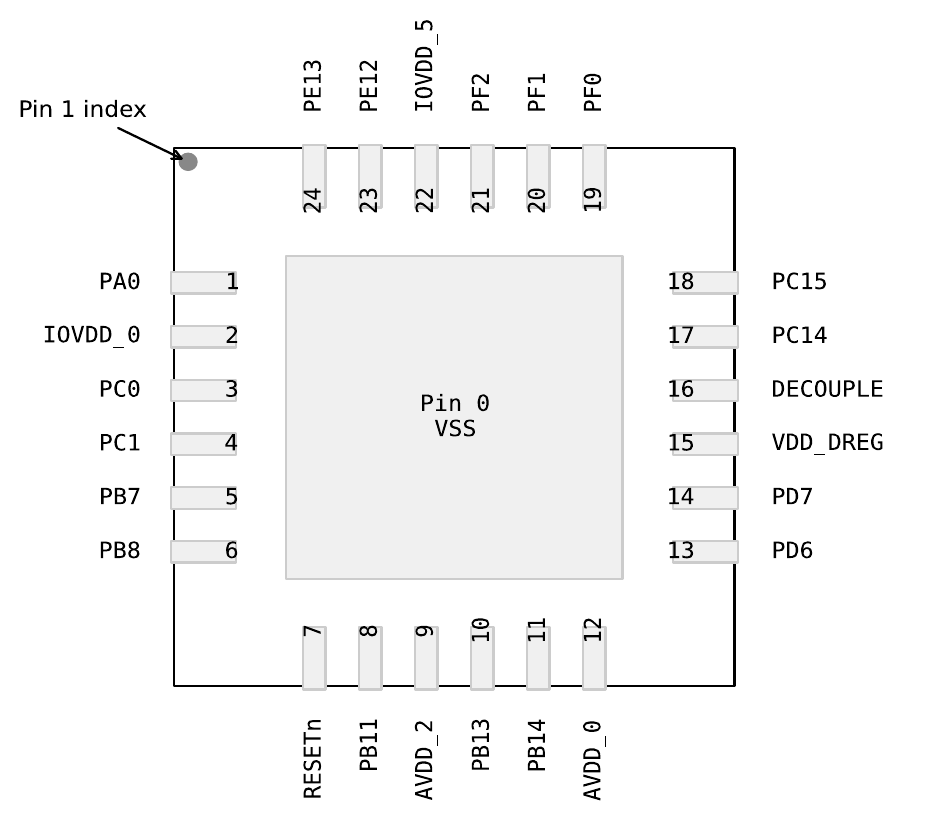
\includegraphics[width=0.65\textwidth, keepaspectratio]{imatges/pinout.png}
 \caption{Pinout pels microcontroladors EFM32ZG, EFM32HG i EFM32TG amb encapsulat QFN24 (extret de \cite[72]{EFM32TGDS}).}
 \label{fig:pinout}
\end{figure}


